\documentclass[
11pt, 
english, 
singlespacing, % Single line spacing
table, % To enable tabular operations.
openany, % To enforce using next available page thus preventing creation of blank pages.
%draft, 
%liststotoc, % To add the list of figures/tables/etc to the table of contents
%toctotoc, % To add the main table of contents to the table of contents
%parskip, % To add space between paragraphs
%nohyperref, % To not load the hyperref package
headsepline, % To get a line under the header
%chapterinoneline, % To place the chapter title next to the number on one line
%consistentlayout, % To change the layout of the declaration, abstract and acknowledgements pages to match the default layout
]{ProjectReport} % The class file specifying the document structure

\usepackage[utf8]{inputenc} % Required for inputting international characters
\usepackage[T1]{fontenc} % Output font encoding for international characters

\usepackage{mathpazo} % Use the Palatino font by default

\usepackage[backend = biber, style = ieee, natbib = true,]{biblatex} % Use the biber backend with the authoryear citation style (which resembles APA)

\addbibresource{biblio.bib} % The filename of the bibliography

\usepackage[autostyle=true]{csquotes} % Required to generate language-dependent quotes in the bibliography

\usepackage{caption}

\usepackage{subcaption} % To use subfigure marker.
\usepackage{mathtools} % To write discontinuous functions and other mathematical formulations.

%----------------------------------------------------------------------------------------
%	MARGIN SETTINGS
%----------------------------------------------------------------------------------------

\geometry{
	paper=a4paper, % Change to letterpaper for US letter
	inner=2.5cm, % Inner margin
	outer=3.8cm, % Outer margin
	bindingoffset=.5cm, % Binding offset
	top=1.5cm, % Top margin
	bottom=1.5cm, % Bottom margin
	%showframe, % Uncomment to show how the type block is set on the page
}

\graphicspath{ {./Figures/} }

%----------------------------------------------------------------------------------------
%	REPORT INFORMATION
%----------------------------------------------------------------------------------------

\thesistitle{\href{https://github.com/t6nand/source-separation}{Source Separation based on Deep Learning}} % Your Project Report title, this is used in the title and abstract, print it elsewhere with \ttitle
\supervisor{Ms. Han Li} % Your supervisor's name, this is used in the title page, print it elsewhere with \supname
\examiner{Prof. Dr.-Ing. Bernhard U. Seeber} % Your examiner's name, this is not currently used anywhere in the template, print it elsewhere with \examname
\degree{MSCE} % Your degree name, this is used in the title page and abstract, print it elsewhere with \degreename
\author{Tapan \textsc{Sharma}} % Your name, this is used in the title page and abstract, print it elsewhere with \authorname

\subject{Project Lab course in Audio Information Processing} % Your subject area, this is not currently used anywhere in the template, print it elsewhere with \subjectname
\university{\href{http://www.tum.de}{Technische Universität München}} % Your university's name and URL, this is used in the title page and abstract, print it elsewhere with \univname
\department{\href{https://www.msce.ei.tum.de/index.php}{Master of Science in Communications Engineering}} % Your department's name and URL, this is used in the title page and abstract, print it elsewhere with \deptname
\group{\href{https://www.ei.tum.de/aip/startseite/}{Chair of Audio Signal Processing}} % Your research group's name and URL, this is used in the title page, print it elsewhere with \groupname
\faculty{\href{https://www.ei.tum.de/startseite/}{Faculty of Electrical Engineering and Information Technology}} % Your faculty's name and URL, this is used in the title page and abstract, print it elsewhere with \facname

\AtBeginDocument{
\hypersetup{pdftitle=\ttitle} % Set the PDF's title to your title
\hypersetup{pdfauthor=\authorname} % Set the PDF's author to your name
}

\begin{document}

\frontmatter % Use roman page numbering style (i, ii, iii, iv...) for the pre-content pages

\pagestyle{plain} % Default to the plain heading style until the thesis style is called for the body content

%----------------------------------------------------------------------------------------
%	TITLE PAGE
%----------------------------------------------------------------------------------------

\begin{titlepage}
 
\includegraphics[width=5em]{Logo_TUM} % University logo
\begin{center}

\vspace*{.05\textheight}
{\scshape\LARGE \univname\par}\vspace{1.2cm} % University name
\textsc{\Large Project Report}\\[0.5cm] % Thesis type

\HRule \\[0.4cm] % Horizontal line
{\huge \bfseries \ttitle\par}\vspace{0.4cm} % Thesis title
\HRule \\[1.5cm] % Horizontal line
 
\begin{minipage}[t]{0.4\textwidth}
\begin{flushleft} \large
\emph{Author:}\\
{\authorname} % Author name
\end{flushleft}
\end{minipage}
\begin{minipage}[t]{0.4\textwidth}
\begin{flushright} \large
\emph{Supervisor:} \\
{\supname} % Supervisor name  
\end{flushright}
\end{minipage}\\[3cm]

\begin{minipage}[t]{0.4\textwidth}
\begin{center}
\emph{Examiner:} \\
{\examname} % Examiner's name  
\end{center}
\end{minipage}\\[3cm]
 
\vfill

\groupname\\\facname\\[3cm] % Research group name and department name
 
\vfill

{\large \today}\\[4cm] % Date
 
\vfill
\end{center}
\end{titlepage}

%----------------------------------------------------------------------------------------
%	Declaration of Originality
%----------------------------------------------------------------------------------------
\begin{originality}
\addchaptertocentry{\originalityname}
This is to certify that the project titled \textbf{“Source Separation based on Deep Learning”} is my original work and is being submitted to the chair of the \enquote{\textbf{Audio Information Processing}} of the \enquote{\textbf{Faculty of Electrical and Information Technology}} in the \enquote{\textbf{Technische Universität München}}. This report has not been submitted earlier either to this University or to any other University/Institution for the fulfillment of the requirement of a course of study.\\
\\
\textit{Name}: \textbf{Tapan Sharma}\\
\textit{Place}: \textbf{Munich}\\
\textit{Date}: \textbf{12th July, 2019}\\
\end{originality} 

%----------------------------------------------------------------------------------------
%	ACKNOWLEDGEMENT PAGE
%----------------------------------------------------------------------------------------

\begin{acknowledgements}
\addchaptertocentry{\acknowledgementname} % Add the abstract to the table of contents
I would first of all like to thank the \enquote{Chair of Audio Information Processing} under the leadership of Prof. Dr.-Ing. Bernhard U. Seeber for making this project lab course available to the masters students as a module particularly in the curriculum program of MSCE (Master of Science in Communication Engineering).\par
I would also like to thank our project supervisor Ms. Han Li who structured and organised the problem statement for the project very clearly and also motivated us to take on the project work with well defined goals to achieve. Her guidance has been in particular of great help to me in improving my work. She pointed us to the right direction in terms of articles, websites and toolboxes which turned out to be of great help to us.\par
In the end, this project would not have seen timely completion without the help of my project mate Mr. Md. Toaha Umar. His insights in our discussions were very fruitful and helped me deepen my understanding and get a new perspective to approach solving some problems. In all, working with him has helped me a lot in my peer learning. 
\end{acknowledgements}

%----------------------------------------------------------------------------------------
%	ABSTRACT PAGE
%----------------------------------------------------------------------------------------

\begin{abstract}
\addchaptertocentry{\abstractname} % Add the abstract to the table of contents
This report presents an implementation and evaluation of an end-to-end system for speech enhancement based source separation, in the monaural voice recordings. Speech Enhancement is achieved by applying a ratio mask to a time-frequency representation of the input signal and through a subsequent reconstruction for the estimated clean speech signal. The mask is estimated from the noisy mixture input data using deep learning machines which are trained on a dataset obtained by additive mixing of recordings of the clean speech and the different sources of noise at a particular signal-to-noise ratio. The expected intelligibility of the reconstructed audio is compared using the intelligibility metric STOI (Short-Time Objective Intelligebility). The quality of estimated clean speech post processing, is compared using the quality metric PESQ (Perceptual Evaluation of Speech Quality), as recommended by the ITU (International Telecommunication Union). We discover that a deep convolutional neural network based learning machines, achieve a superior performance at speech enhancement using the cochleagram as the training data along with the time-frequency masks based on cochleagrams when compared to other deep learning models working on acoustic features and time-frequency masks as their training data.
\end{abstract}


%----------------------------------------------------------------------------------------
%	LIST OF CONTENTS/FIGURES/TABLES PAGES
%----------------------------------------------------------------------------------------
\tableofcontents % Prints the main table of contents
\listoffigures
\listoftables


%----------------------------------------------------------------------------------------
%	ABBREVIATIONS
%----------------------------------------------------------------------------------------

\begin{abbreviations}{ll} % Include a list of abbreviations (a table of two columns)

\textbf{STFT} & \textbf{S}hort-\textbf{T}ime \textbf{F}ourier \textbf{T}ransform\\
\textbf{ERB} & \textbf{E}quivalent \textbf{R}ectangular \textbf{B}andwidth\\
\textbf{STOI} & \textbf{S}hort-\textbf{T}ime \textbf{O}bjective \textbf{I}ntelligibility\\
\textbf{PESQ} & \textbf{P}erceptual \textbf{E}valuation of \textbf{S}peech \textbf{Q}uality\\
\textbf{MOS} & \textbf{M}ean \textbf{O}pinion \textbf{S}core\\
\textbf{LQO} & \textbf{L}istening \textbf{Q}uality \textbf{O}bjective\\
\textbf{PESQMOS} & \textbf{P}erceptual \textbf{E}valuation of \textbf{S}peech \textbf{Q}uality \textbf{M}ean \textbf{O}pinion \textbf{S}core\\
\textbf{MOSLQO} & \textbf{M}ean \textbf{O}pinion \textbf{S}core \textbf{L}istening \textbf{Q}uality \textbf{O}bjective\\
\textbf{DNN} & \textbf{D}eep \textbf{N}eural \textbf{N}etwork\\
\textbf{CNN} & \textbf{C}onvolutional \textbf{N}eural \textbf{N}etwork\\
\textbf{LSTM} & \textbf{L}ong \textbf{S}hort-\textbf{T}erm \textbf{M}emory\\
\textbf{IRM} & \textbf{I}deal \textbf{R}atio \textbf{M}ask\\
\textbf{GFCC} & \textbf{G}ammatone \textbf{F}requency \textbf{C}epstral \textbf{C}oefficients\\
\textbf{MFCC} & \textbf{M}el-\textbf{F}requency \textbf{C}epstral \textbf{C}oefficients\\
\textbf{t-f} & \textbf{t}ime-\textbf{f}requency\\
\textbf{RMSE} & \textbf{R}oot \textbf{M}ean \textbf{S}quare \textbf{E}rror\\
\textbf{reLU} & \textbf{re}ctified \textbf{L}inear \textbf{U}nit\\

\end{abbreviations}


%----------------------------------------------------------------------------------------
%	SYMBOLS
%----------------------------------------------------------------------------------------

\begin{symbols}{lll} % Include a list of Symbols (a three column table)

$t$ & time & \si{\second} \\
$f$ & frequency & \si{\hertz} \\
$S(t,f)$ & log spectral energy of clean speech signal &  dB per t-f frame \\
$N(t,f)$ & log spectral energy of noise signal &  dB per t-f frame \\

\end{symbols}


%----------------------------------------------------------------------------------------
%	REPORT CONTENT - CHAPTERS
%----------------------------------------------------------------------------------------

\mainmatter % Begin numeric (1,2,3...) page numbering

\pagestyle{thesis} % Return the page headers back to the "thesis" style

% Include the chapters of the thesis as separate files from the Chapters folder

% Chapter 1

\chapter{Introduction} % Main chapter title

\label{Chapter1} % For referencing the chapter elsewhere, use \ref{Chapter1} 

%----------------------------------------------------------------------------------------

% Define some commands to keep the formatting separated from the content 
\newcommand{\keyword}[1]{\textbf{#1}}
\newcommand{\tabhead}[1]{\textbf{#1}}
\newcommand{\code}[1]{\texttt{#1}}
\newcommand{\file}[1]{\texttt{\bfseries#1}}
\newcommand{\option}[1]{\texttt{\itshape#1}}

%----------------------------------------------------------------------------------------

\section{Why Source Separation?}
For a healthy person it is an incredible feat to tune into a single conversation in a crowded room while being completely oblivious to background noise and other conversations that happen simultaneously. This ability for a person to solve the \enquote{Cocktail Party Problem}\cite{wiki:cock} is remarkable and very natural as a human. However, an estimated 5\% of the world’s population suffers from disabling hearing loss \cite{ref:who}. For the 466 million affected people the ability to perceive speech especially in the presence of background noise is significantly impaired. Since the perception of speech is crucial for being able to communicate verbally, this impairment has profound social and emotional consequences for the sufferers \cite{ref:who}.\par 
Current hearing aids offer only limited relief as they cannot distinguish between speech and background noise and will simply opt to amplify both signals. This does not greatly help with the intelligibility. Hence, the focus should be on designing an “intelligent” system that can distinguish between the conversation and disruptive background noise in order to provide an improvement to hearing aids. It is not unconceivable that such systems would also be of great help to the people with a normal and healthy hearing considering the fact that listening to someone in a loud environment is still detrimental to the hearing. \par An estimated half of all cases of hearing loss in adults are caused by exposure to excessively loud noise \cite{ref:deb}. A system that can remove loud background noise but allow for unhindered conversation might therefore help prevent such cases of hearing loss.\par
This project report contributes to these goals by comparing different implementations of supervised deep learning systems that can learn to enhance speech from background noise in monaural (single microphone) recordings. \par
%----------------------------------------------------------------------------------------

\section{Historical Work}
The first approach to solve the Cocktail Party Problem was using the concept of \enquote{\textbf{Spectral Subtraction}}\cite{ref:spec_sub}. This approach makes an assumption that the clean speech signal has been corrupted by statistically independent additive noise. The power spectrum of the noise signal can be recovered approximately for stationary noise by taking the average of multiple signal frames. This estimated power spectrum is then subtracted from the mixed signal spectrum, keeping the phase information intact. The resulting subtraction results in less noise in the estimated signal but the quality of such estimation also tends to deteriorate considering the fact that many tones tend to appear and disappear rapidly in the reconstructed signal.\par
The idea to use a deep learning machine in order to filter out background noise from speech recordings goes back three decades. In 1988 Tamura and Waibel \cite{ref:shin} showed that a four-layer feed-forward neural network could successfully be used to directly separate the waveforms of Japanese speech recordings from computer lab background noise. This network is small by the standards of today, but took weeks of training on a supercomputer of its time. The authors note that the perceived quality of the filtered audio was higher, but that intelligiblity did not improve.\par 
Artificially adding noise to existing audio recordings is routinely used in supervised training of automatic speech recognition systems in order to improve their robustness towards environmental noise \cite{ref:awni}. Chen, Jitong and Wang \cite{ref:tong} follow an approach rooted in the computational auditory scene analysis (CASA). The idea is to predict an “Ideal Ratio Mask” (IRM) that describes the proportion of speech to noise energy in a frequency band at a given time. When the IRM is known, the clean speech signal can be reconstructed from the noisy signal by weighting each time frequency unit of the noisy recording according to its speech content.\par
Huang, Kim, Hasegawa-Johnson and Smargdis further improve this approach by presenting a framework for separating arbitrarily many sources using recurrent neural networks (RNNs) using a discriminative training criterion\cite{ref:rnn}. They also move the time-frequency masking operation directly into a layer of the neural network in order to jointly optimize the network with the masking function.
\par

%----------------------------------------------------------------------------------------

\section{Limitations}
There are several assumptions made in this project which limit the direct application of the results in a real time situations. These limitations can however be overcome by acquiring more training data.
\begin{itemize}
\item While the recordings of noise included complex interactions of the sound sources with the environment like factory noise, waterfalls, engine noise, etc., the speech examples were considered from relataively simpler scenarios without any interaction of sound sources with the real world conditions. Hence, many effects like reverberated speech are not modeled.
\item \textit{Lombard Effect \cite{wiki:lom}}: It is the ability of humans to alter their speaking style in order to allow for efficient verbal communication in a noisy environment. This too has not been considered. Hence, there is likely to be a mismatch between the prediction of the data considered in the project with the real world data.
\end{itemize}
% Chapter 2

\chapter{Methodology} % Main chapter title

\label{Chapter2} % For referencing the chapter elsewhere, use \ref{Chapter2} 

%----------------------------------------------------------------------------------------

\section{Supervised learning architecture for speech enhancement}
Supervised learning is the machine learning task of learning a function that maps an input to an output based on example input-output pairs \cite{wiki:sl}. In supervised learning, each example is a pair consisting of an input object and a desired output value (also called the supervisory signal). A supervised learning algorithm analyzes the training data and produces an inferred function, which can be used for mapping new examples.\par
The idea of using supervised learning for speech-enhancement involves using the training data consisting of audio features as input object and the desired t-f mask as an output value during the training phase (See figure: \ref{fig:training_layout}). This would enable a deep learning model to learn a function to model the training data. The trained deep learning model can then be used on a testing dataset that would only involve audio features as input to the trained deep learning model. Post training phase, the deep learning model would then predict the t-f mask for the input audio features (See figure: \ref{fig:testing_layout}).\par
\begin{figure}
\centering
\begin{subfigure}{.5\textwidth}
  \centering
  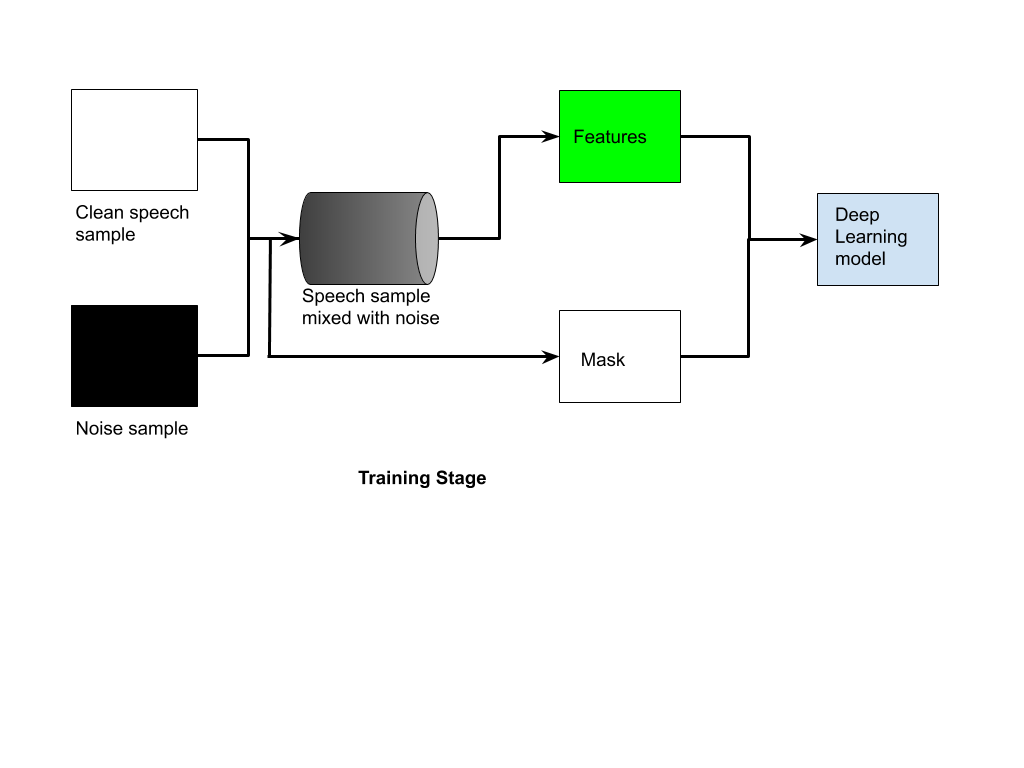
\includegraphics[width=1.25\linewidth]{training_layout}
  \caption{Training Stage Layout}
  \label{fig:training_layout}
\end{subfigure}%
\begin{subfigure}{.5\textwidth}
  \centering
  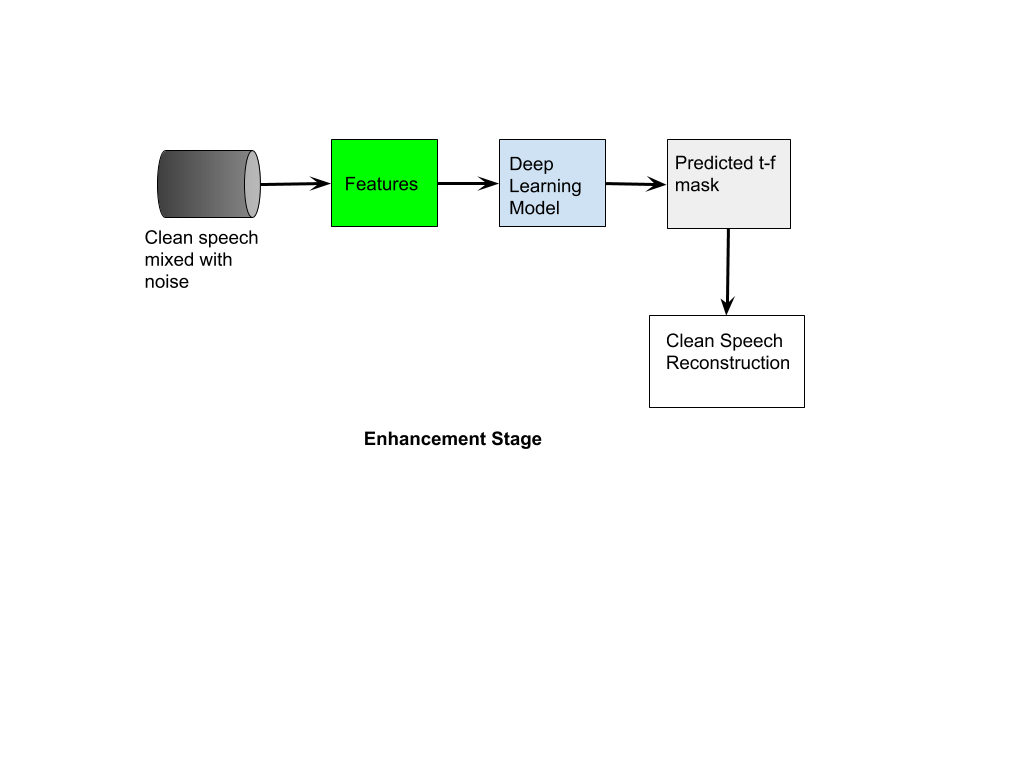
\includegraphics[width=1.25\linewidth]{testing_layout}
  \caption{Testing Stage Layout}
  \label{fig:testing_layout}
\end{subfigure}
\caption{Deep Learning based speech enhancement layouts}
\label{fig:layouts}
\end{figure}
%----------------------------------------------------------------------------------------
\section{Dataset}
Dataset forms the most important part of any supervised learning problem. For the experiments in this project, only the speech portion, which consists of read speech (TIMIT recordings), and the set of noises(MUSAN recordings), which ranges from beeps emitted from technical equipment, to ambient sounds such as rain, road , factory noise, etc) were considered. All of the files are available in \enquote{.wav} format, are single channel, and are 16 bit sample PCM encoded. All recordings are downsampled to 8kHz sampling rate to speed up the training phase.

\begin{itemize}
\item \textbf{Clean Speech Dataset}:\\
\textbf{\href{http://www.ldc.upenn.edu/Catalog/CatalogEntry.jsp?catalogId=LDC93S1}{TIMIT}}: This corpus \cite{ref:timit} consists of a total of 1700 sentences spoken by roughly 630 speakers of eight major dialects of American English. TIMIT corpus includes time-aligned orthographic, phonetic and word transcriptions as well as a 16-bit, 16kHz speech waveform file for each utterance. To speed up the training in our case however, these samples were downsampled to 8kHz. Corpus design was a joint effort among the Massachusetts Institute of Technology (MIT), SRI International (SRI) and Texas Instruments, Inc. (TI). The speech was recorded at TI, transcribed at MIT and verified by the National Institute of Standards and Technology (NIST).
\item \textbf{Noise Dataset}:\\
\textbf{\href{https://www.openslr.org/17/}{MUSAN}}: This is a corpus of music, speech, and noise recordings \cite{ref:musan2015}. This dataset consists of music, speech recordings in twelve different languages, and a large set of naturally occuring and technical noises. Its primary intention is that of being a training corpus for voice activity detection. We considered the noise sub set of this corpus which amounts to around 6 hours of the duration.
\end{itemize}

\subsection{Generation of Noisy Mixture}
During training phase, the clean speech sample was mixed with a randomly chosen noise sample after making both samples of same duration and at the same amplitude level, i.e. both clean speech and noise samples were first normalised to have same amplitude and then added together. The mixing procedure has been depicted as a flow chart in the figure \ref{fig:gen_mix}.

\begin{figure}[!htbp]
\centering
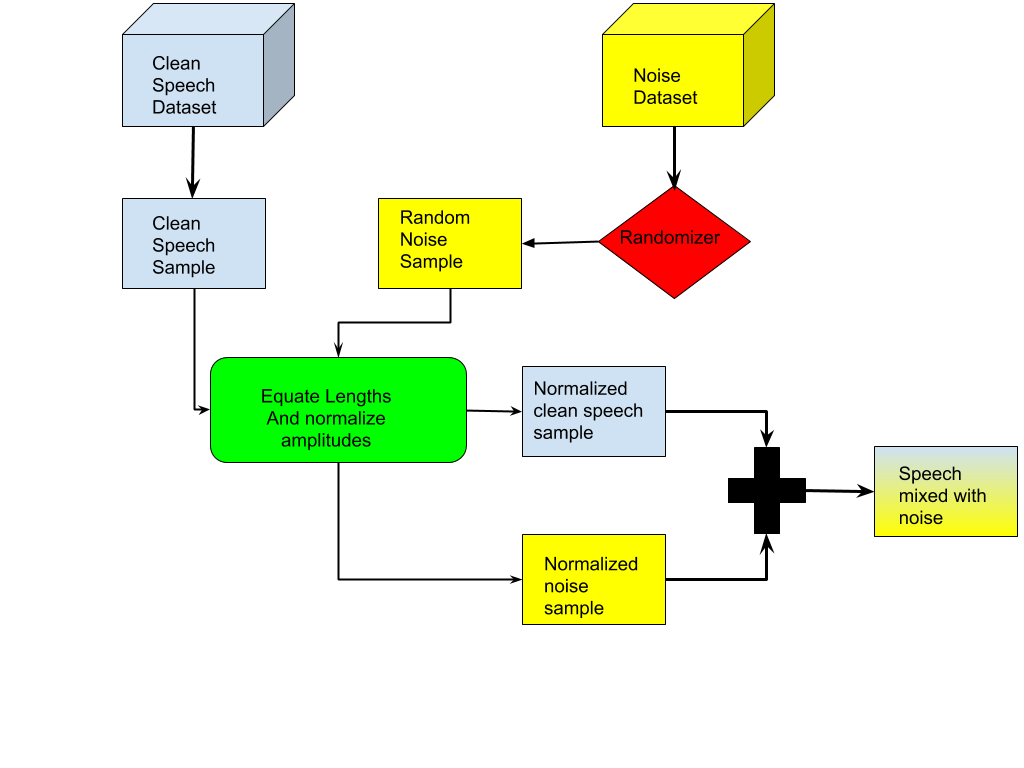
\includegraphics[width=1.15\linewidth]{gen_mix}
\caption{Generation of Noisy speech samples}
\label{fig:gen_mix}
\end{figure}

%---------------------------------------------------------------------------
\section{Features}
In machine learning and pattern recognition, a feature is an individual measurable property or characteristic of a phenomenon being observed \cite{wiki:feat}. Choosing informative, discriminating and independent features is a crucial step for effective algorithms in pattern recognition, classification and regression. \par Features as input and learning machines play complementary roles in supervised learning. When features are discriminative,they place less demand on the learning machine in order to perform a task successfully. On the other hand, a powerful learning machine places less demand on features.\par We conducted a study to examine different acoustic features for supervised speech enhancement:

\subsection{\textbf{Spectrogram}}
A spectrogram is a visual representation of the spectrum of frequencies of a signal as it varies with time. Spectrogram for an audio is constructed by combining the STFT at subband levels. Audio samples at 8 K\si{\hertz} are divided into frames of 30 m\si{\second}. Hence, each frame has 240 samples for which STFT is calculated. An overlap of 60 samples in adjacent frames is also used to reduce the effect of windowing. Combining STFT for all subband frames gives a spectrogram which can then be used as the training data and for generating spectrogram masks (See figure: \ref{fig:spect}).
\begin{figure}
\centering
\begin{subfigure}{.4\textwidth}
  \centering
  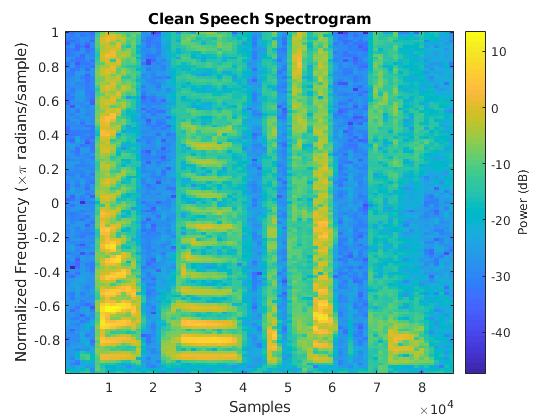
\includegraphics[width=1.1\linewidth]{clean_spect}
  \caption{Clean Speech Spectrogram}
  \label{fig:clean_spect}
\end{subfigure}%
\begin{subfigure}{.4\textwidth}
  \centering
  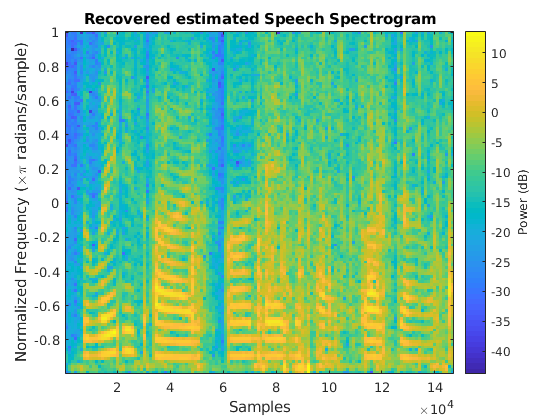
\includegraphics[width=1.1\linewidth]{mix_spect}
  \caption{Noisy mixture spectrogram}
  \label{fig:mix_spect}
\end{subfigure}
\begin{subfigure}{.4\textwidth}
  \centering
  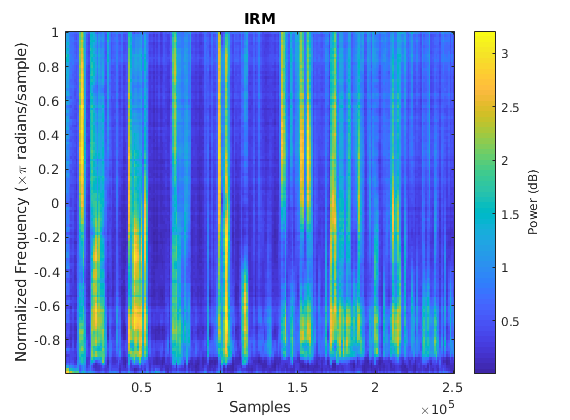
\includegraphics[width=1.1\linewidth]{IRM_spect}
  \caption{IRM - by learning model}
  \label{fig:irm_spect}
\end{subfigure}
\begin{subfigure}{.4\textwidth}
  \centering
  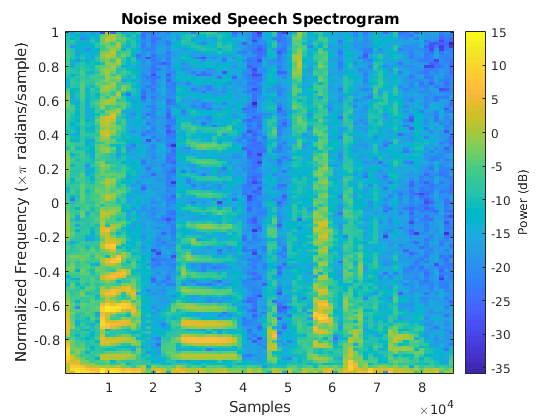
\includegraphics[width=1.1\linewidth]{estimated_spect}
  \caption{Estimated speech spectrogram}
  \label{fig:est_spect}
\end{subfigure}
\caption{Different stages of spectrogram during speech enhancement}
\label{fig:spect}
\end{figure}

\subsection{\textbf{GFCC}}
GFCC (Gammatone Frequency Cepstral Coefficients) are the gammatone-domain cepstrum based audio feaures. Being a cepstral property, it is a spectral representation of the spectrum of a time domain audio signal which has been filtered using a gammatone filterbank. These features are calculated at subband levels for frames of length 30ms. For an audio sampled at 8K\si{\hertz} rate, this imply 240 samples per frame. To reduce the effect of windowing, an overlap of 60 samples in adjacent frames is considered. This method to calculate GFCC, the rate of change of GFCC called GFCC delta and rate of change of GFCC delta, called GFCC double delta is described in \ref{fig:gfcc_extraction}. In all 13 gammatone frequency cepstral coefficients were considered (See figure: \ref{fig:gfcc_plot} \cite{mathworks:gtcc}).  

\begin{figure}
\centering
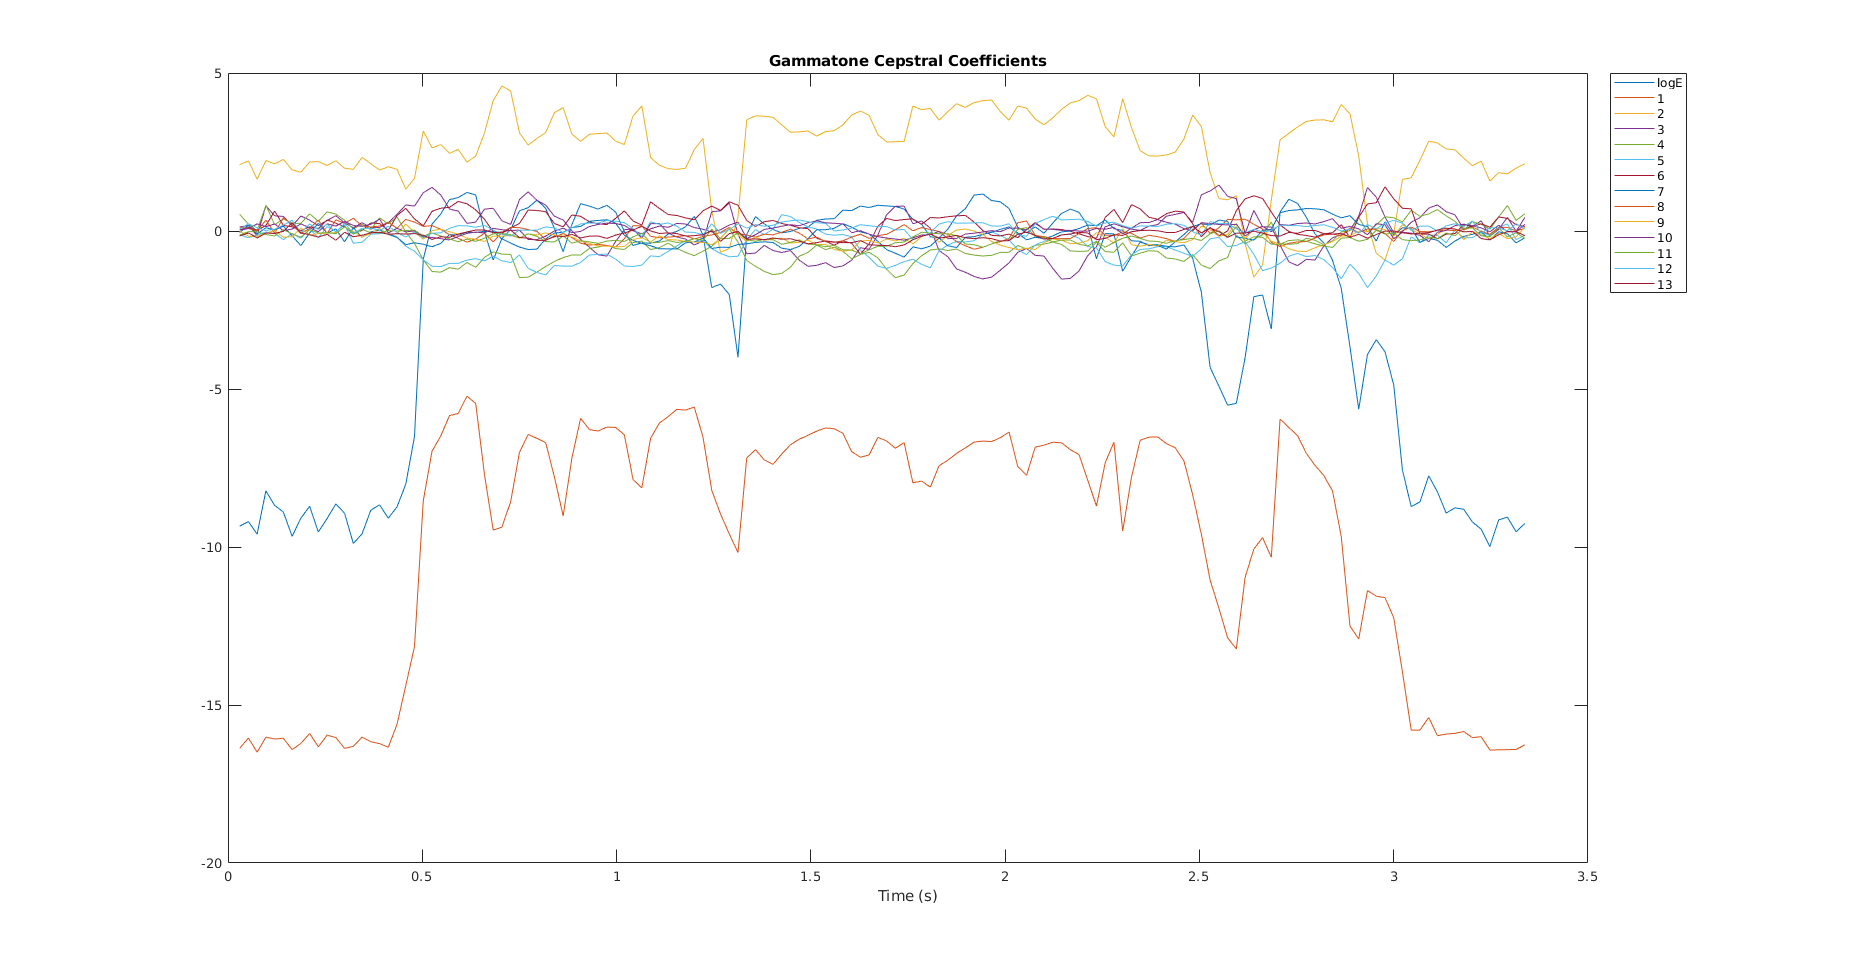
\includegraphics[width=1.15\linewidth]{gfcc_plot}
\caption{Typical GFCC plot with log energy and 13 coefficients}
\label{fig:gfcc_plot}
\end{figure}

\begin{figure}
\centering
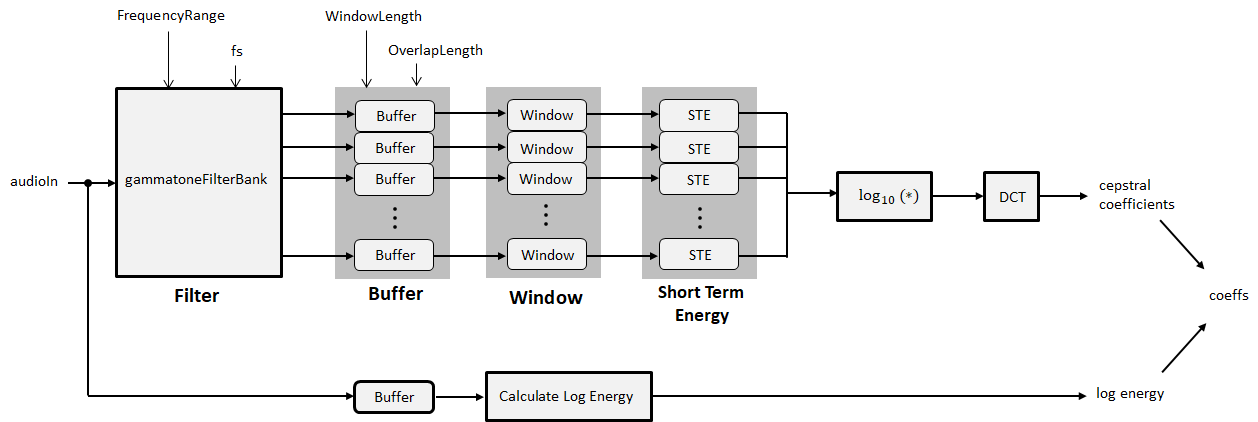
\includegraphics[width=1.2\linewidth]{gtcc_algorithm}
\caption{GFCC Extraction}
\label{fig:gfcc_extraction}
\end{figure}

\begin{figure}
\centering
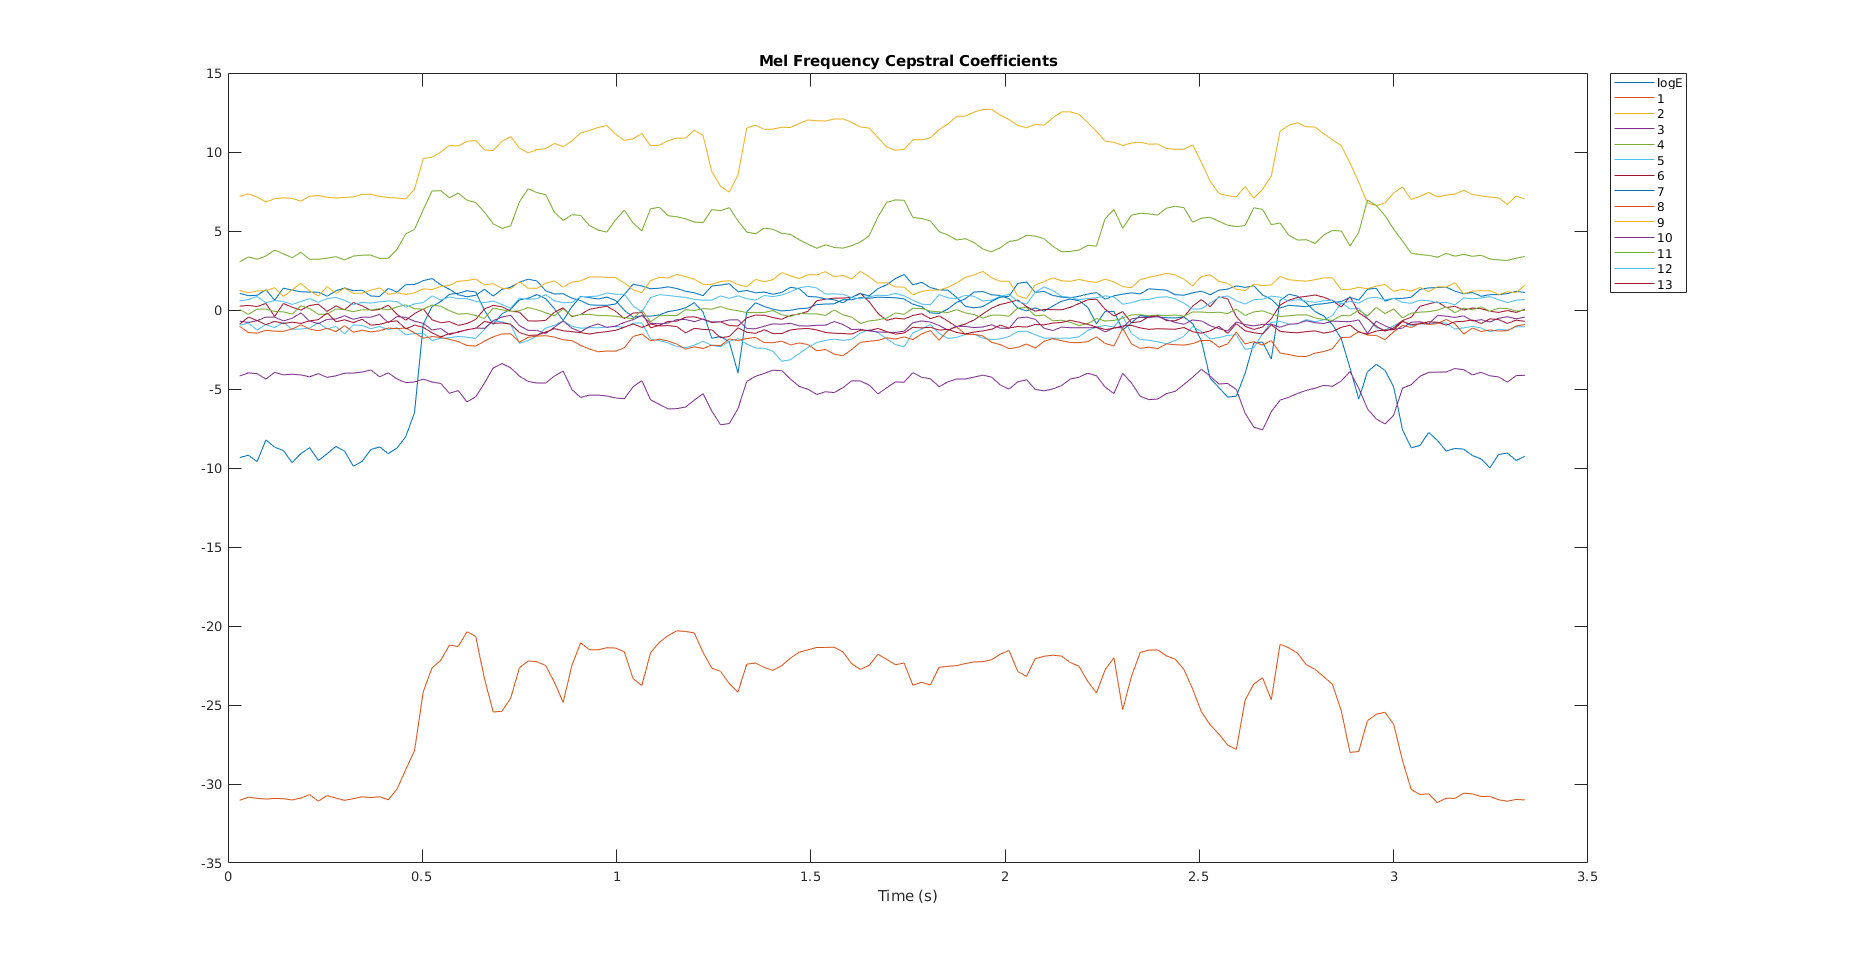
\includegraphics[width=1.25\linewidth]{mfcc_plot}
\caption{Typical MFCC plot with log enery and 13 coefficients}
\label{fig:mfcc_plot}
\end{figure}

\subsection{\textbf{MFCC}}
MFCC (Mel-Frequency Cepstral Coefficients) are the Mel-domain cepstrum based audio features. It is a spectral representation of the spectrum of a time domain audio signal which has been filtered using a mel-frequency filterbank. The MFCC is calculated by splitting the entire data into overlapping segments. These features are calculated at subband levels for frames of length 30ms. For an audio sampled at 8K\si{\hertz} rate, this imply 240 samples per frame. To reduce the effect of windowing, an overlap of 60 samples in adjacent frames is considered (See figure:\ref{fig:mfcc_extraction} \cite{mathworks:mfcc}). Using this methodology, the mel frequency cepstral coefficients, log energy values, cepstral delta, and the cepstral delta-delta values for each segment is calculated. In all 13 mel-frequency cepstral coefficients were considered (See figure: \ref{fig:mfcc_plot})

\begin{figure}
\centering
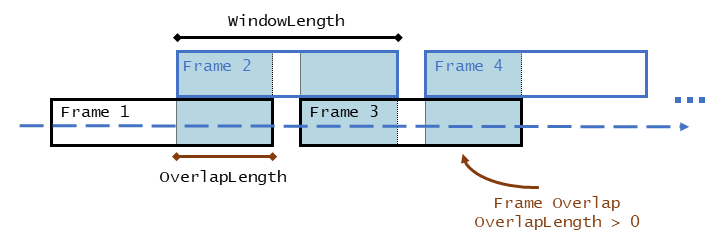
\includegraphics[width=1.1\linewidth]{mfcc_audioframes}
\caption{Audio Feature Extraction using sub-band audio frames}
\label{fig:mfcc_extraction}
\end{figure}

\subsection{\textbf{Pitch}}
Pitch estimates fundamental frequency of audio signal (See figure: \ref{fig:pitch_plot}). The pitch values are also estimated for an audio at sub-band levels for frames of length 30ms. For an audio sampled at 8K\si{\hertz} rate, this imply 240 samples per frame. To reduce the effect of windowing, an overlap of 60 samples in adjacent frames is considered (See figure:\ref{fig:mfcc_extraction}\cite{mathworks:mfcc}).

\begin{figure}
\centering
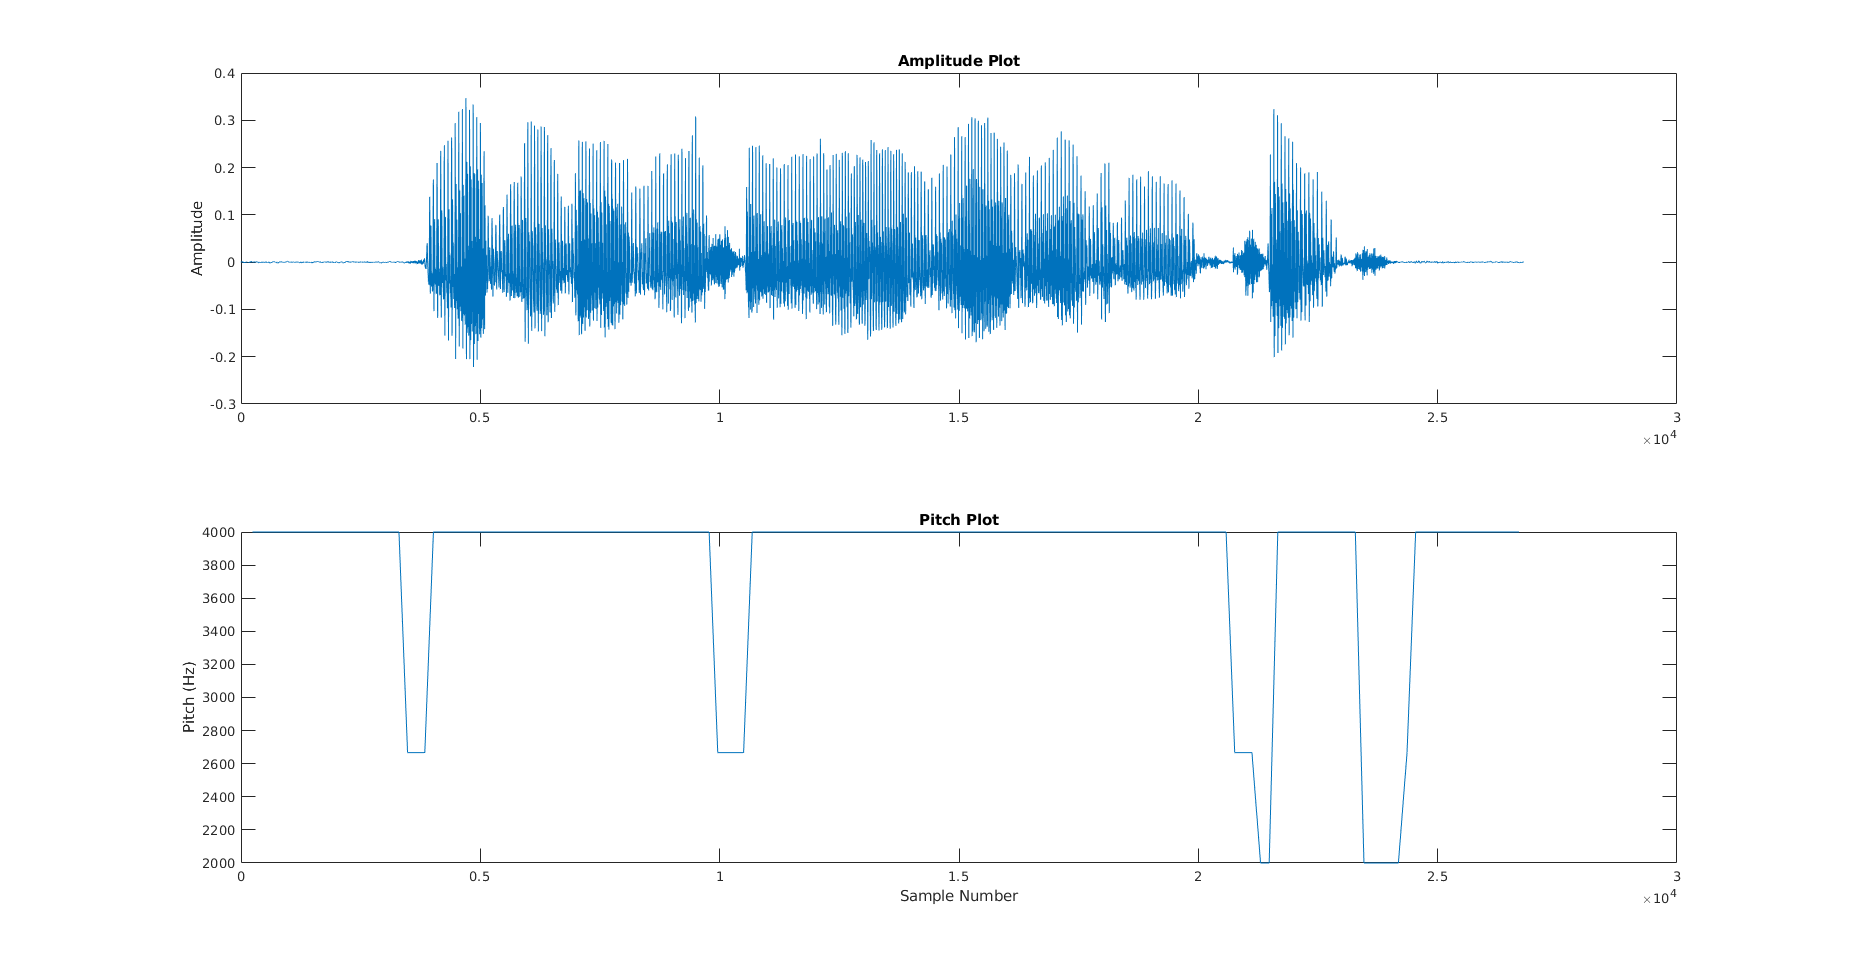
\includegraphics[width=1.2\linewidth]{pitch_plot}
\caption{Pitch plot for an audio waveform}
\label{fig:pitch_plot}
\end{figure}

\subsection{\textbf{Cochleagram}}
This is a representation of a  time-domain audio waveform in a t-f domain but is different from the spectrogram (See figure:\ref{fig:coch}). It is computed using an array of band pass filters that each model the frequency selectivity and nerve response of a single hair cell. Keeping this in mind, a 64 channel Gammatone filter bank as an array of band pass filters is used to estimate cochleagram.
Cochleagram evaluation involves using ERB (Equivalent Rectangular Bandwidth) as a psychoacoustic measure for approximating the frequency-dependent bandwidth of the filters in human hearing. The bandwidth of the rectangular bandpass filter is chosen such that it has the same peak and passes the same amount of power for an input of white noise.
\begin{figure}
\centering
\begin{subfigure}{.4\textwidth}
  \centering
  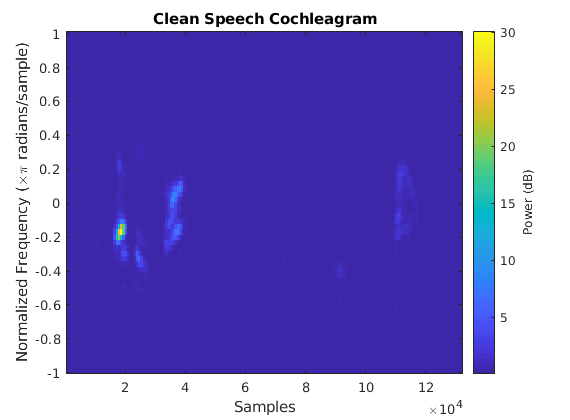
\includegraphics[width=1.1\linewidth]{clean_coch}
  \caption{Clean speech cochleagram}
  \label{fig:clean_coch}
\end{subfigure}%
\begin{subfigure}{.4\textwidth}
  \centering
  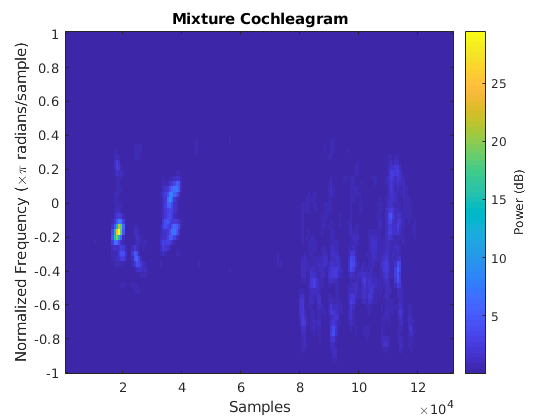
\includegraphics[width=1.1\linewidth]{mix_coch}
  \caption{Noisy mixture cochleagram}
  \label{fig:mix_coch}
\end{subfigure}
\begin{subfigure}{.4\textwidth}
  \centering
  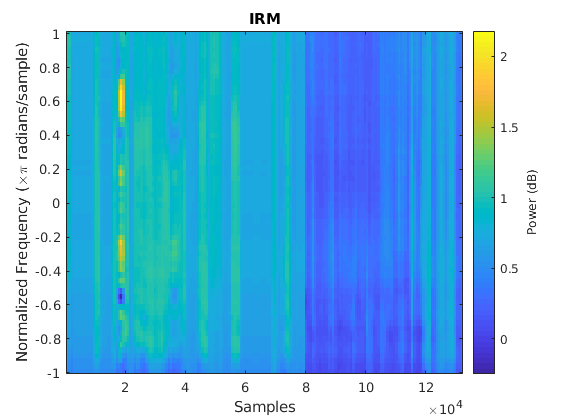
\includegraphics[width=1.1\linewidth]{irm_coch}
  \caption{IRM - by learning model}
  \label{fig:irm_coch}
\end{subfigure}
\begin{subfigure}{.4\textwidth}
  \centering
  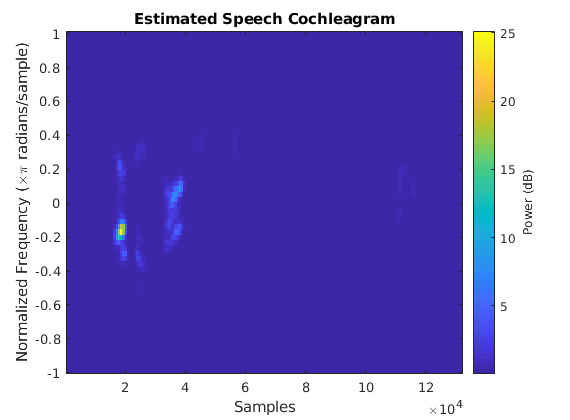
\includegraphics[width=1.1\linewidth]{estimated_coch}
  \caption{Estimated speech cochleagram}
  \label{fig:estimated_coch}
\end{subfigure}
\caption{Different stages of cochleagram during speech enhancement}
\label{fig:coch}
\end{figure}
%----------------------------------------------------------------------------------------

\section{Training Targets}
In supervised speech enhancement, defining a proper training target is important for learning and generalization. There are mainly two groups of training targets, i.e., masking-based targets and mapping-based targets. Masking-based targets describe the t-f relationships of clean speech to background interference, while mapping-based targets correspond to the spectral representations of clean speech. We focused on masking based training targets with a particular emphasis on usage of an \textbf{IRM} as a training target.\\
\subsection{IRM} 
IRM (Ideal Ratio Mask) is a soft mask \cite{ref:irm} which can be thresholded into a binary mask based on some local thresholding criterion. IRM is defined as:
\begin{equation}
IRM = \bigg( \frac{S(t,f)^2}{S(t,f)^2 + N(t,f)^2} \bigg)^\beta
\label{eq:irm}
\end{equation}
where $$S(t,f)^2$$ and $$N(t,f)^2$$ denote speech energy and noise energy within a T-F unit, respectively. The tunable parameter $$\beta$$ scales the mask, and is commonly chosen to 0.5. With the square root the IRM preserves the speech energy with each T-F unit, under the assumption that \textit{S(t,f)} and \textit{N(t,f)} are uncorrelated. Without the root the IRM in \ref{eq:irm} is similar to the classical Wiener filter, which is the optimal estimator of target speech in the power spectrum. An example of the IRM is shown in \ref{fig:irm_spect} and \ref{fig:irm_coch}.


 
% Chapter 3
\chapter{Deep Learning Models} % Main chapter title

\label{Chapter3} % For referencing the chapter elsewhere, use \ref{Chapter3} 

%----------------------------------------------------------------------------------------
In this project, deep learning models based on following deep neural networks were considered:\\
\begin{itemize}
\item \textbf{Feedforward Deep Neural Network}
\item \textbf{Deep Convolutional Neural Network}
\end{itemize}
%----------------------------------------------------------------------------------------
\section{Baseline DNN model}
A baseline deep neural network model was considered with the following architecture (See figure: \ref{fig:dnn_0}):
\begin{figure}[!htbp]
\centering
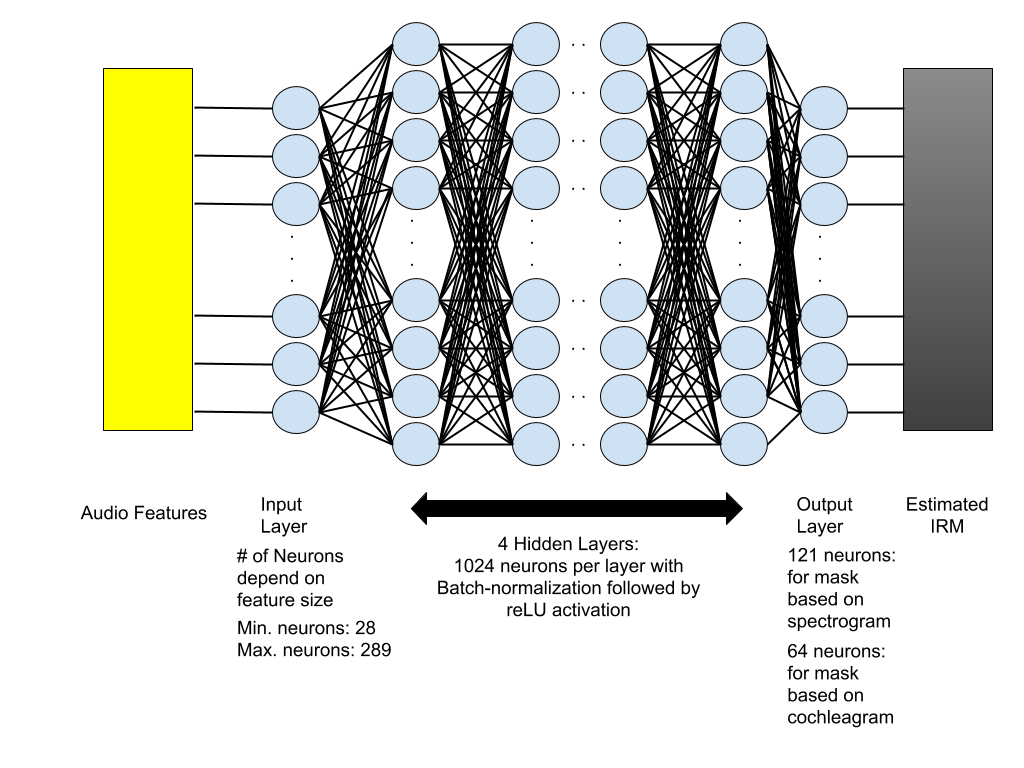
\includegraphics[width=1.2\linewidth]{dnn_0}
\caption{A Baseline feedforward deep neural network with 5 layers}
\label{fig:dnn_0}
\end{figure}
\begin{itemize}
\item \textbf{Image Input Layer}:\\
This layer accepts the feature data as a 2-D or 3-D input. The number of neurons is this layer depends on the dimension size of the features. For the different combination of features on which this DNN was trained, the minimum number of input neurons were 28 for only GFCC and MFCC features. The maximum number of neurons were 289 for a combination of Spectrogram, GFCC,GFCC Delta ,GFCC double delta, MFCC, MFCC Delta, MFCC double delta and Pitch features.
\item \textbf{Hidden Layers}:\\
Four hidden layers were used with the following properties:
\begin{itemize}
\item \textbf{Fully Connected Layer}:\\
This layer connect every neuron in one layer to every neuron in another layer \cite{wiki:cnn}.
\item \textbf{Batch Normalization}:\\
Since the activations are constantly changing during training for the intermediate layers, this slows down the training process because each layer must learn to adapt themselves to a new distribution in every training step. This problem is known as \enquote{\textit{internal covariate shift}}. Batch normalization is a method used to normalize the inputs of each layer, in order to fight the internal covariate shift problem \cite{wiki:batch}. During training time, a batch normalization layer does the following:
\begin{enumerate}
\item Calculate the mean and variance of the layers input.
\item Normalize the layer inputs using the previously calculated batch statistics.
\item Scale and shift in order to obtain the output of the layer.
\end{enumerate}
\item \textbf{reLU activation}:\\
The rectified linear unit activation function is a piecewise linear function that will output the input directly if is positive, otherwise, it will output zero \cite{wiki:relu}. This thus helps in overcoming \enquote{\textit{vanishing gradient problem}} (See 3.3) often encountered with traditional tanh or sigmoid activations. reLU activation applys the function  $$f(x)=max(0,x)$$ where \textit{x} is the output calculated post weight multiplication and bias addition at a given layer. 
\end{itemize}
\item \textbf{Output Layer}:\\
Output layer is a fully connected layer with regression operation. The number of neurons in this layer is equal to the dimension of the IRM to estimate. For a spectrogram based IRM, the number of output neurons are 121 and for a cochleagram based IRM, the number of output neurons are 64. Regression operation tries to minimize a cost function to model the feature set with respect to the IRM to estimate. The metric used for optimisation is Root Mean Square Error (RMSE) to minimize the intended cost function for modeling the training data.
\end{itemize}

\subsection{Experiments with baseline DNN}
Baseline DNN was used to identify the best feature set for speech enhancement with an emphasis on finding simpler features with improvement in the intelligibility and quality with reduced computing resource consumption. Experiments were divided into two categories based on training targets, viz \enquote{IRM based on spectrograms} and \enquote{IRM based on cochleagram}. Baseline DNN was trained for noisy mixtures at 0 SNR and -2 SNR respectively.\\

\begin{enumerate}
\item \textbf{IRM based on spectrograms}:\\
\begin{itemize}
\item \textbf{Intelligibility}:\\
STOI performance for different combination of audio features is listed in the table \ref{tab:dnn_0_stoi}. Following inferences can be made:\\ 
\begin{enumerate}
\item \textbf{Comparison between worst performing and best performing features}:\\
As evident from the table \ref{tab:dnn_0_stoi}, the gain in intelligibility from the worst performing and the best performing feature set is  \enquote{\textbf{2.5\%}} for SNR 0 and \enquote{\textbf{1.3\%}} for SNR -2.\\ 
\item \textbf{Comparison of intelligibility with noisy audios}:\\
On comparing with the intelligibilty scores of the original noisy mixture for the best performing feature set (See table: \ref{tab:stoi_mix}) the gain in intelligibility scores for SNR 0 is \enquote{\textbf{10.9\%}} and for SNR -2 is \enquote{\textbf{14.9\%}}.\\
\end{enumerate}
\begin{table}[!htbp]
\centering
\begin{tabular}{ |p{12cm}|p{1.7cm}|p{1.7cm}|  }
\hline
\textbf{Features} & \multicolumn{2}{|c|}{\textbf{STOI}} \\
\hline
\cellcolor{black} & SNR 0 & SNR -2 \\
\hline
Spectrogram & 0.81	& 0.76\\
\hline
Spectrogram, MFCC, MFCC Delta, MFCC delta delta & 0.80	& 0.77\\
\hline
Spectrogram, Pitch &	0.79 & 0.76\\
\hline
Spectrogram, GFCC, GFCC Delta, GFCC delta delta & 0.80	& 0.77\\
\hline
Spectrogram, GFCC, GFCC Delta, GFCC delta delta, MFCC, MFCC Delta, MFCC delta delta &	0.80 & 0.77\\
\hline
GFCC, MFCC & 0.79 & 0.76\\
\hline
Spectrogram, GFCC, MFCC & 0.80 & 0.77\\
\hline
\rowcolor[HTML]{ADD8E6}GFCC, GFCC Delta, GFCC delta delta & 0.81 & 0.77\\
\hline
GFCC, GFCC Delta, GFCC delta delta, MFCC, MFCC delta, MFCC delta delta &	0.81 & 0.77\\
\hline
Spectrogram, GFCC, GFCC delta, GFCC delta delta, MFCC, MFCC delta, MFCC delta delta, Pitch & 0.79 & 0.76\\
\hline
MFCC, MFCC delta, MFCC delta delta & 0.80 & 0.77\\
\hline
\end{tabular}
\caption{STOI performance: Baseline, IRM based on spectrogram}
\label{tab:dnn_0_stoi}
\end{table}

\item \textbf{Quality}:\\
PESQ performance for different combination of audio features is listed in the table \ref{tab:dnn_0_pesq}.Following inferences can be made:\\
\begin{enumerate}
\item \textbf{Comparison of quality gain from worst to best performing feature set}:\\
The quality gain from the worst performing feature set to the best performing feature set is \enquote{\textbf{9.9\%}} for \textbf{PESQMOS} and \enquote{\textbf{11.5\%}} for \textbf{MOSLQO}  for SNR 0. For SNR -2 the gain in quality is \enquote{\textbf{6.6\%}} for \textbf{PESQMOS} and \enquote{\textbf{8.8\%}} for \textbf{MOSLQO} respectively.
\item \textbf{Comparison of quality gain from noisy mixtures}:\\
It's also important to compare the gain in quality in estimated speech signal as compared to the quality scores of the noisy mixture which  has been tabulated in \ref{tab:pesq_mix} for  the best performing feature set, for SNR 0 and -2 respectively. Hence, comparing both tables gives us a gain in quality of \enquote{\textbf{10.5\%}} for \textbf{PESQMOS} and \enquote{\textbf{10.9\%}} for \textbf{MOSLQO} at SNR 0 and the gain in quality of \enquote{\textbf{9.8\%}} for \textbf{PESQMOS} and \enquote{\textbf{11.3\%}} for \textbf{MOSLQO} at SNR -2 respectively.
\end{enumerate} 
\begin{table}[!htbp]
\centering
\begin{tabular}{ |p{8cm}|p{1.7cm}|p{1.7cm}|p{1.7cm}|p{1.7cm}|  }
\hline
\textbf{Features} & \multicolumn{4}{|c|}{\textbf{PESQ}}\\
\hline
\cellcolor{black} & \multicolumn{2}{|c|}{SNR 0} & \multicolumn{2}{|c|}{SNR -2}\\
\hline
\cellcolor{black} & PESQMOS & MOSLQO & PESQMOS & MOSLQO\\
\hline
Spectrogram	& 2.11	& 1.82	& 2.10	& 1.81\\
\hline
Spectrogram,MFCC,MFCC delta,MFCC delta delta	& 2.31	& 2.03	& 2.21	& 1.93\\
\hline
Spectrogram,Pitch	& 2.23	& 1.95	& 2.18	& 1.93\\
\hline
\cellcolor{yellow}Spectrogram,GFCC,GFCC delta,GFCC delta delta	& 2.29	& 1.99	& \cellcolor{yellow}2.24	& \cellcolor{yellow}1.97\\
\hline
Spectrogram,GFCC,GFCC delta,GFCC delta delta MFCC,MFCC delta,MFCC delta delta	& 2.30	& 2.02	& 2.19	& 1.92\\
\hline
GFCC,MFCC	& 2.26	& 1.96	& 2.16	& 1.88\\
\hline
Spectrogram,GFCC,MFCC	& 2.29	& 2.00	& 2.22	& 1.95\\
\hline
\cellcolor[HTML]{ADD8E6}GFCC,GFCC delta,GFCC delta delta	& \cellcolor[HTML]{ADD8E6}2.32	& \cellcolor[HTML]{ADD8E6}2.03	& 2.20	& 1.92\\
\hline
GFCC,GFCC delta,GFCC delta delta MFCC,MFCC delta,MFCC delta delta	& 2.28	& 1.99	& 2.19	& 1.90\\
\hline
Spectrogram,GFCC,GFCC delta,GFCC delta delta MFCC,MFCC delta,MFCC delta delta,Pitch	& 2.19	& 1.90	& 2.16	& 1.87\\
\hline
MFCC,MFCC delta,MFCC delta delta	& 2.26	& 1.98	& 2.13	& 1.85\\
\hline
\end{tabular}
\caption{PESQ performance: Baseline, IRM based on spectrogram}
\label{tab:dnn_0_pesq}
\end{table}

\begin{table}[!htbp]
\centering
\begin{tabular}{ |p{8cm}|p{1.7cm}|p{1.7cm}|p{1.7cm}|p{1.7cm}|  }
\hline
\textbf{Features} & \multicolumn{4}{|c|}{\textbf{PESQ}}\\
\hline
\cellcolor{black} & \multicolumn{2}{|c|}{SNR 0} & \multicolumn{2}{|c|}{SNR -2}\\
\hline
Noise mixed speech samples & 2.10 & 1.83 & 2.04 & 1.73\\
\hline
\end{tabular}
\caption{PESQ values for noisy mixture}
\label{tab:pesq_mix}
\end{table}
 
\end{itemize}
\item \textbf{IRM based on cochleagrams}:\\
\begin{itemize}
\item \textbf{Intelligibility}:\\
STOI performance for different combination of audio features is listed in the table \ref{tab:dnn_0_stoi_1}. Following inferences can be made.\\
\begin{enumerate}
\item \textbf{Comparison with the IRM based on Spectrogram}:\\
As evident from the table \ref{tab:dnn_0_stoi_1}, the gain in intelligibility score for the best performing feature sets is \enquote{\textbf{1.2\%}} when compared to the best performing feature set for the IRM based on spectrogram for SNR 0 and for SNR -2 the intelligibility scores are the same for both the cases.
\item \textbf{Comparison from the worst to best performing feature set}:\\
The gain in intelligibility score from worst performing feature set to the best performing feature set is by \enquote{\textbf{6.5\%}} for SNR 0 and \enquote{\textbf{6.9\%}} for SNR -2.\\ 
\item \textbf{Gain in intelligibility from noisy mixtures}:\\
For the best perfroming feature set, when compared to the original noisy mixture's intelligibility (see table: \ref{tab:stoi_mix}), the gain is \enquote{\textbf{12.3\%}} for SNR 0 and for SNR -2, the gain in intelligibility is \enquote{\textbf{14.9\%}}.\\ 
\end{enumerate}
Hence, it highlights a better performance than the IRM based on spectrograms for the intelligibility gains.

\item \textbf{Quality}:\\
PESQ performance for different combination of audio features is listed in the table \ref{tab:dnn_0_pesq_2}. Following observations can be made:\\ 
\begin{enumerate}
\item \textbf{Comparison with IRM based on spectrogram}:\\
As it's evident from the table \ref{tab:dnn_0_pesq_2}, the quality scores are better as compared to IRM based on spectrogram for the best performing feature sets in the both cases by around 2.1\% for 0 SNR and by around 3.1\% for -2 SNR considering PESQMOS as quality metric for the best performing feature set. 
\item \textbf{Comparison of quality gain from worst to best performing feature set}:\\
Quality gain from the worst performing feature set to the best performing feature set is by \enquote{\textbf{9.7\%}} for \textbf{PESQMOS} and \enquote{\textbf{11.9\%}} for \textbf{MOSLQO} at SNR 0. At SNR -2 the gain in quality is \enquote{\textbf{13.8\%}} for \textbf{PESQMOS} and  \enquote{\textbf{14.3\%}} for \textbf{MOSLQO}.
\item \textbf{Comparison with the quality of noisy mixtures}:\\
On comparing for quality gain from the noisy mixtures for the best performing feature set as tabulated in the table \ref{tab:pesq_mix}, there is a gain of \enquote{\textbf{12.8\%}} for \textbf{PESQMOS} and \enquote{\textbf{13.1\%}} for \textbf{MOSLQO} at SNR 0 and the gain in quality of \enquote{\textbf{13.2\%}} for \textbf{PESQMOS} and \enquote{\textbf{15.6\%}} for \textbf{MOSLQO} at SNR -2 respectively.
\end{enumerate}
This highlights the importance of \enquote{\textbf{Cochleagram}} as  training data for low SNR scenarios and also highlight the overall improvement in quality when using cochleagram based masks as compared to spectrogram based masks during training.
\end{itemize}
\end{enumerate}

\begin{table}[!htbp]
\centering
\begin{tabular}{ |p{12cm}|p{1.7cm}|p{1.7cm}|  }
\hline
\textbf{Features} & \multicolumn{2}{|c|}{\textbf{STOI}} \\
\hline
\cellcolor{black} & SNR 0 & SNR -2 \\
\hline
\rowcolor[HTML]{ADD8E6}Cochleagram	& 0.82	& 0.77\\
\hline
GFCC,GFCC delta,GFCC delta delta	& 0.78	& 0.73\\
\hline
GFCC,GFCC delta,GFCC delta delta MFCC,MFCC delta,MFCC delta delta	& 0.77	& 0.74\\
\hline
MFCC,MFCC delta,MFCC delta delta	& 0.78	& 0.75\\
\hline
GFCC,MFCC	& 0.78	& 0.74\\
\hline
\end{tabular}
\caption{STOI performance: Baseline, IRM based on cochleagram}
\label{tab:dnn_0_stoi_1}
\end{table}

\begin{table}[!htbp]
\centering
\begin{tabular}{ |p{8cm}|p{1.7cm}|p{1.7cm}|p{1.7cm}|p{1.7cm}|  }
\hline
\textbf{Features} & \multicolumn{4}{|c|}{\textbf{PESQ}}\\
\hline
\cellcolor{black} & \multicolumn{2}{|c|}{SNR 0} & \multicolumn{2}{|c|}{SNR -2}\\
\hline
\cellcolor{black} & PESQMOS & MOSLQO & PESQMOS & MOSLQO\\
\hline
\cellcolor[HTML]{ADD8E6}Cochleagram	& \cellcolor[HTML]{ADD8E6}2.37	& \cellcolor[HTML]{ADD8E6}2.07	& \cellcolor{yellow}2.31	& \cellcolor{yellow}2.00\\
\hline
GFCC,GFCC delta,GFCC delta delta	& 2.23	& 1.92	& 2.05	& 1.75\\
\hline
GFCC,GFCC delta,GFCC delta delta MFCC,MFCC delta,MFCC delta delta	& 2.21	& 1.91	& 2.09	& 1.80\\
\hline
MFCC,MFCC delta,MFCC delta delta	& 2.16	& 1.85	& 2.09	& 1.82\\
\hline
GFCC,MFCC	& 2.27	& 1.96	& 2.06	& 1.77\\
\hline
\end{tabular}
\caption{PESQ performance: Baseline, IRM based on cochleagram}
\label{tab:dnn_0_pesq_2}
\end{table}


\begin{table}[!htbp]
\centering
\begin{tabular}{ |p{12cm}|p{1.7cm}|p{1.7cm}|  }
\hline
\textbf{Features} & \multicolumn{2}{|c|}{\textbf{STOI}} \\
\hline
\cellcolor{black} & SNR 0 & SNR -2 \\
\hline
Noise Mixed Speech Samples	& 0.73	& 0.67\\
\hline
\end{tabular}
\caption{STOI values for Noise Mixed speech samples}
\label{tab:stoi_mix}
\end{table}
%--------------------------------------------------------------------------------------
\section{DNN model based on biased sigmoid activation}
Another deep neural network model was considered with the following architecture (See figure: \ref{fig:dnn_1}):
\begin{itemize}
\item \textbf{Image Input Layer}:\\
This layer accepts the feature data as a 2-D or 3-D input. The number of neurons is this layer depends on the dimension size of the features just as with the baseline model.
\item \textbf{Hidden Layers}:\\
Four hidden layers were used with the following properties:
\begin{itemize}
\item \textbf{Fully Connected Layer}:\\
This layer connect every neuron in one layer to every neuron in another layer.
\item \textbf{Biased Sigmoid Layer}:\\
This layer is an alteration on a sigmoid layer which uses a sigmoid activation function (See figure: \ref{fig:sigmoid}) to overcome \enquote{\textit{vanishing gradient problem}}. The number of neurons in these layers are twice the number of neurons in the input layer. Sigmoid function, squishes a large input space into a small input space between 0 and 1. Therefore, a large change in the input of the sigmoid function will cause a small change in the output. Hence, the derivative becomes small. This causes the neural network to have a reduced learning with the gradients not able to reach the optimization points over time. The biased sigmoid activation layer overcomes this problem by enforcing the sigmoid function to operate on it's linear part where the derivative of the function is significantly better than the case when the sigmoid function operates closer to the region of 0 and 1. Hence, the biased sigmoid layer is able to overcome the \enquote{\textit{Vanishing Gradient Problem}}. The purpose of using this layer is to compare it's performance with the reLU activation used in the baseline DNN as discussed in the previous section. 
\item \textbf{Batch Normalization}:\\
As discussed in the previous section, this layer helps in overcoming\enquote{\textit{internal covariate shift}}. It does so by normalizing the inputs of each layer.
\item \textbf{Dropout Layer}:\\
This layer works on a tunable parameter called the \enquote{\textit{Dropout Probability}}. During the training phase, the proportion of neurons as defined by the parameter \enquote{\textit{Dropout Probability}} on a particular layer are deactivated. This improve generalization because it forces a layer to learn with different neurons the same "concept". Hence, this is used to prevent overfitting of the training data, where a learning machine has an ability to model the training data but performs poorly on the testing data. During the prediction phase however, the dropout is deactivated.
\end{itemize}
\begin{figure}[!htbp]
\centering
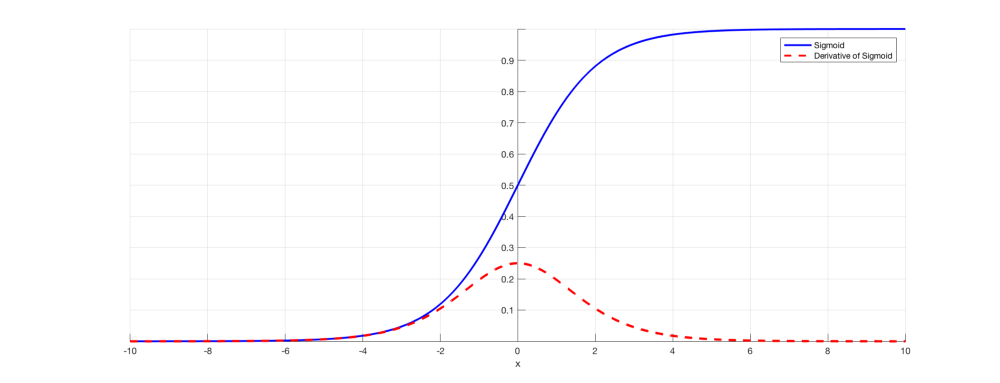
\includegraphics[width=1.1\linewidth]{sigmoid}
\caption{Sigmoid activation function.}
\label{fig:sigmoid}
\end{figure}
\item \textbf{Output Layer}:\\
Output layer is a fully connected layer with biased sigmoid activation and  regression operation. The number of neurons in this layer is equal to the dimension of the IRM to estimate. For a spectrogram based IRM, the number of output neurons are 121 and for a cochleagram based IRM, the number of output neurons are 64. Biased sigmoid layer tries to prevent \enquote{\textit{Vanishing Gradient Problem}} followed by a regression operation, which tries to minimize a cost function to model the feature set with respect to the IRM to estimate by using RMSE as an optimization metric.
\end{itemize}
\begin{figure}[!htbp]
\centering
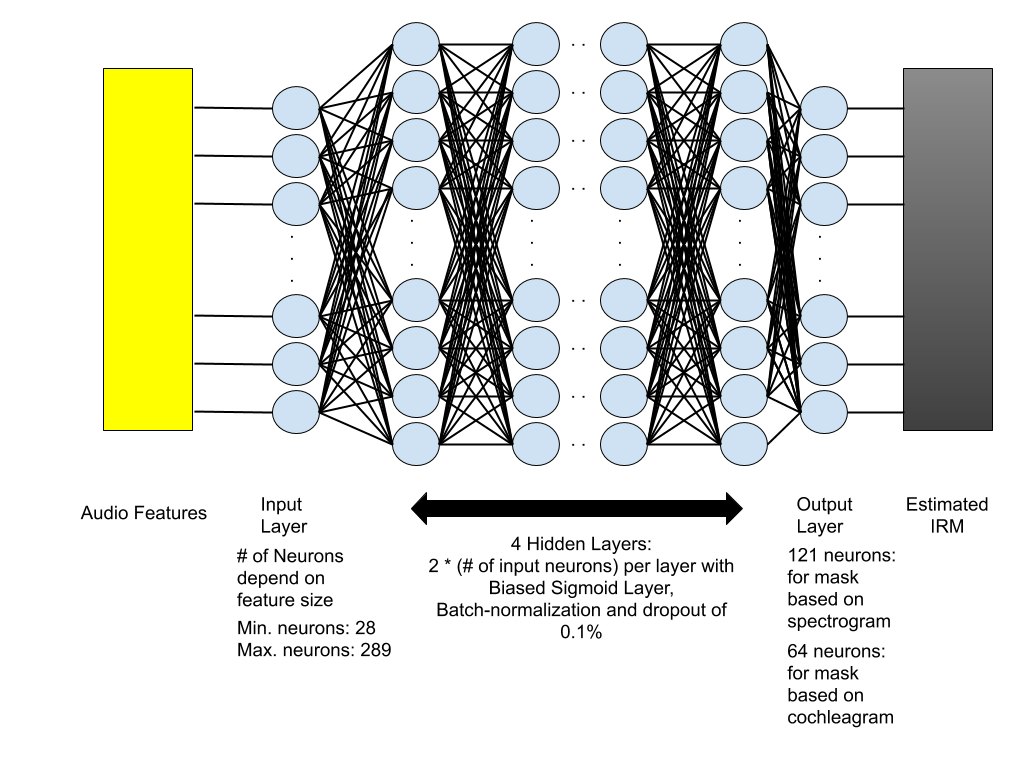
\includegraphics[width=1.2\linewidth]{dnn_1}
\caption{A feedforward deep neural network with 5 layers and biased sigmoid activation}
\label{fig:dnn_1}
\end{figure}

\subsection{Experiments with the DNN using biased activation}
Using the results from the baseline DNN, experiments were conducted using the best performing feature sets with the baseline DNN. Similar to the baseline DNN, experiments were divided into two categories based on training targets, viz “IRM based on spectrograms” and “IRM based on cochleagram”. Training was done for noisy mixtures at 0 SNR and -2 SNR respectively.
\begin{enumerate}
\item \textbf{IRM based on Spectrogram}
\begin{itemize}
\item \textbf{Intelligibility}:\\
STOI performance for different combination of audio features is listed in
the table \ref{tab:dnn_1_stoi_1}. Following observations can be made:\\
\begin{enumerate}
\item \textbf{Comparison with the baseline DNN}:\\
As it's evident from the table \ref{tab:dnn_1_stoi_1}, there is no significant improvement in the intelligiblity scores as compared to the baseline DNN's performance tabulated in the table \ref{tab:dnn_0_stoi_1}. Infact for the best performning feature set, the intelligibilty score is reduced by \enquote{\textbf{1.25\%}} for SNR 0. Although the intelligibility for SNR -2 as compared to the baseline DNN is the same for the same feature set.
\item \textbf{Comparison of intelligibility gain from worst to the best performing features}:\\
The improvement in intelligibility for the feature sets used for this experiment from the worst performing to the best performing set is by \enquote{\textbf{2.5\%}} for SNR 0 and for SNR -2, the improvement is \enquote{\textbf{4\%}}.
\item \textbf{Comparison with the noisy mixtures}:
The intelligibility gains as compared to the noisy mixtures (see table: \ref{tab:stoi_mix}) is \enquote{\textbf{9.6\%}} for SNR 0 and for SNR -2 the gain is of \enquote{\textbf{14.9\%}}.
\end{enumerate}
The best performing feature set in this case was still found out to be \enquote{\textbf{GFCC, GFCC delta, GFCC delta delta}} for both SNR 0 and SNR -2 which is similar to the performance of this feature set with the baseline DNN for SNR 0 whereas in the case of the baseline DNN for -2 SNR, the best feature set was \enquote{\textbf{Spectrogram, GFCC, GFCC delta, GFCC delta delta}}. This reflects a strong correlation of GFCC related feature set with the IRM based on spectrogram. However, overall the intelligibilty performance shows no significant improvement as compared to the baseline DNN for this deep learning model.

\begin{table}[!htbp]
\centering
\begin{tabular}{ |p{12cm}|p{1.7cm}|p{1.7cm}|  }
\hline
\textbf{Features} & \multicolumn{2}{|c|}{\textbf{STOI}} \\
\hline
\cellcolor{black} & SNR 0 & SNR -2\\
\hline
Spectrogram	& 0.79	& 0.76\\
\hline
Spectrogram,GFCC,GFCC delta,GFCC delta delta	& 0.80	& 0.76\\
\hline
Spectrogram,GFCC,MFCC	& 0.78	& 0.77\\
\hline
\rowcolor[HTML]{ADD8E6}GFCC,GFCC delta,GFCC delta delta	& 0.80	& 0.77\\
\hline
GFCC,GFCC delta,GFCC delta delta MFCC,MFCC delta,MFCC delta delta	& 0.79	& 0.74\\
\hline
\end{tabular}
\caption{STOI performance: DNN2, IRM based on spectrogram}
\label{tab:dnn_1_stoi_1}
\end{table}

\item \textbf{Quality}:\\
PESQ performance for different combination of audio features is listed in
the table \ref{tab:dnn_1_pesq_1}. Following inferences can be made:\\
\begin{enumerate}
\item \textbf{Comparison with the baseline DNN}:\\
From the table \ref{tab:dnn_1_pesq_1}, and comparing the PESQ scores with the baseline DNN documented in the table \ref{tab:dnn_0_pesq}, the scores show deterioration of the quality. The best performing feature set \enquote{\textit{Spectrogram,GFCC,GFCC delta,GFCC delta delta}}, shows detereoration of \enquote{\textbf{0.8\%}} for \textbf{PESQMOS} score and detereoration of \enquote{\textbf{0.9\%}} for the \textbf{MOSLQO} score when compared to the performance of the best performing feature set found for the baseline DNN at SNR 0. For SNR -2, the best performing feature set \enquote{\textbf{GFCC, GFCC delta, GFCC delta delta}} showed the detereoration of \enquote{\textbf{1.8\%}} for the \textbf{PESQMOS} score, and the \textbf{MOSLQO} scores were the same at \enquote{1.97}.
\item \textbf{Comparison of quality gain from worst to the best performing feature}:\\
For this experiment the gain of quality from the worst performing feature set to the best performing feature set was of \enquote{\textbf{8.4\%}} for \textbf{PESQMOS} and \enquote{\textbf{5.2\%}} for \textbf{MOSLQO} at SNR 0. At SNR -2, the gain in quality from the worst to the best performing feature set was of \enquote{\textbf{10\%}} for \textbf{PESQMOS} and \enquote{\textbf{8.2\%}} for \textbf{MOSLQO}.
\item \textbf{Comparison with the noisy mixture}:\\
On comparing the quality gain for the best performing feature set in this experiment from the noisy mixture as documented in the table \ref{tab:dnn_1_pesq_1} the gain was \enquote{\textbf{9.5\%}} for \textbf{PESQMOS} and \enquote{\textbf{9.8\%}} for \textbf{MOSLQO} at SNR 0. At SNR -2, the gain was \enquote{\textbf{7.8\%}} for \textbf{PESQMOS} and \enquote{\textbf{11.3\%}} for \textbf{MOSLQO}.
\end{enumerate}
Overall, it can be said that there is no significant improvement when comapred to the quality gain performance of the baseline DNN for this deep learning model.
\begin{table}[!htbp]
\centering
\begin{tabular}{ |p{8cm}|p{1.7cm}|p{1.7cm}|p{1.7cm}|p{1.7cm}|  }
\hline
\textbf{Features} & \multicolumn{4}{|c|}{\textbf{PESQ}}\\
\hline
\cellcolor{black} & \multicolumn{2}{|c|}{SNR 0} & \multicolumn{2}{|c|}{SNR -2}\\
\hline
\cellcolor{black} & PESQMOS & MOSLQO & PESQMOS & MOSLQO\\
\hline
Spectrogram	& 2.21	& 1.91	& 2.17	& 1.90\\
\hline
\cellcolor[HTML]{ADD8E6}Spectrogram,GFCC,GFCC delta,GFCC delta delta	& \cellcolor[HTML]{ADD8E6}2.30	& \cellcolor[HTML]{ADD8E6}2.01	& 2.12	& 1.82\\
\hline
Spectrogram,GFCC,MFCC	& 2.22	& 1.98	& 2.00	& 1.93\\
\hline
\cellcolor{yellow}GFCC,GFCC delta,GFCC delta delta	& 2.28	& 1.99	& \cellcolor{yellow}2.20	& \cellcolor{yellow}1.97\\
\hline
GFCC,GFCC delta,GFCC delta delta MFCC,MFCC delta,MFCC delta delta	& 2.12	& 1.97	& 2.00	& 1.89\\
\hline
\end{tabular}
\caption{PESQ performance: DNN2, IRM based on spectrogram}
\label{tab:dnn_1_pesq_1}
\end{table}
\end{itemize}

\item \textbf{IRM based on Cochleagram}
\begin{itemize}
\item \textbf{Intelligibility}
STOI performance for different combination of audio features is listed in the table \ref{tab:dnn_1_stoi_2}. Following observations can be made:\\
\begin{enumerate}
\item \textbf{Comparison with the baseline DNN}:\\
From the table \ref{tab:dnn_1_stoi_2}, shows a detereoration in the intelligibility score as comapred to the baseline DNN's performance by \enquote{\textbf{2.5\%}} for SNR 0 and for SNR -2, by \enquote{\textbf{1.3\%}} for the best performing feature set.
\item \textbf{Comparison from the worst and the best performing feature set}:\\
Since the intelligibility performance was poor with the feature sets in the previous experiment with IRM based on spectrogram, this experiment was confined to the best performing set of \enquote{\textit{GFCC, GFCC delta, GFCC delta delta}} and \enquote{\textit{Cochleagram}}. Within this experiment, the intelligibility gain from worst performing feature set to the best performing feature set is \enquote{\textbf{3.9\%}} for SNR 0 and for SNR -2, the gain was \enquote{\textbf{5.5\%}}.
\item \textbf{Comparison with the noisy mixtures}:\\
On comparing with the intelligibility of the noisy mixtures (see table: \ref{tab:stoi_mix}), the gain was found out to be \enquote{\textbf{9.6\%}} at 0 SNR and at \enquote{\textbf{13.4\%}} -2 SNR for \enquote{\textit{Cochleagram}} as the better performing feature set in the previous case.
\end{enumerate}
This shows an improvement in intelligibility scores when using IRM based on cochleagram as training target compared to the IRM based on spectrogram which is as per the trend with the baseline DNN as well. However, compared to intelligibility gains provided by the baseline DNN, this deep learning model shows no significant improvement.
\begin{table}[!htbp]
\centering
\begin{tabular}{ |p{12cm}|p{1.7cm}|p{1.7cm}|  }
\hline
\textbf{Features} & \multicolumn{2}{|c|}{\textbf{STOI}} \\
\hline
\cellcolor{black} & SNR 0 & SNR -2\\
\hline
\rowcolor[HTML]{ADD8E6}Cochleagram	& 0.80	& 0.76\\
\hline
GFCC, GFCC delta, GFCC delta delta & 0.77	& 0.72\\
\hline
\end{tabular}
\caption{STOI performance: DNN2, IRM based on cochleagram}
\label{tab:dnn_1_stoi_2}
\end{table}

\item \textbf{Quality}
PESQ performance for the different combination of audio features is listed in the table \ref{tab:dnn_1_pesq_2}. Following inferences can be made:\\
\begin{enumerate}
\item \textbf{Comparison with the baseline DNN}:\\
On comparing the tabulated data from the table \ref{tab:dnn_1_pesq_2}, with the baseline DNN's performance in the table \ref{tab:dnn_0_pesq_2}, for the best performing feature set, there is detereoration in quality by \enquote{\textbf{1.7\%}} for \textbf{PESQMOS} and \enquote{\textbf{0.9\%}} for \textbf{MOSLQO} for SNR 0. For SNR -2, the detereoration is by \enquote{\textbf{1.7\%}} for \textbf{PESQMOS} and \enquote{\textbf{1\%}} for \textbf{MOSLQO}.
\item \textbf{Comparison from the worst to best performing feature set}:\\
Within this experiment the gain in quality from the worst perfroming feature set to the best performing feature set was found out to be \enquote{\textbf{8.1\%}} for \textbf{PESQMOS} and \enquote{\textbf{9.9\%}} for \textbf{MOSLQO} for SNR 0. For SNR -2, the detereoration is by \enquote{\textbf{11.8\%}} for \textbf{PESQMOS} and \enquote{\textbf{13.1\%}} for \textbf{MOSLQO}.
\item \textbf{Comparison with the noisy mixture}:\\
On comapring with the quality of noisy mixtures as tabulated in the table \ref{tab:pesq_mix}, the gain in quality was found out to be \enquote{\textbf{11.2\%}} for \textbf{PESQMOS} and \enquote{\textbf{12.9\%}} for \textbf{MOSLQO} for SNR 0. For SNR -2, the detereoration is by \enquote{\textbf{13.5\%}} for \textbf{PESQMOS} and \enquote{\textbf{13.8\%}} for \textbf{MOSLQO} respectively.
\end{enumerate}
Overall, this too shows no significant improvement in quality gains as comaperd with the gains provided by the baseline DNN.
\begin{table}[!htbp]
\centering
\begin{tabular}{ |p{8cm}|p{1.7cm}|p{1.7cm}|p{1.7cm}|p{1.7cm}|  }
\hline
\textbf{Features} & \multicolumn{4}{|c|}{\textbf{PESQ}}\\
\hline
\cellcolor{black} & \multicolumn{2}{|c|}{SNR 0} & \multicolumn{2}{|c|}{SNR -2}\\
\hline
\cellcolor{black} & PESQMOS & MOSLQO & PESQMOS & MOSLQO\\
\hline
\cellcolor[HTML]{ADD8E6}Cochleagram	& \cellcolor[HTML]{ADD8E6}2.39	& \cellcolor[HTML]{ADD8E6}2.10	& \cellcolor{yellow}2.27	& \cellcolor{yellow}1.98\\
\hline
GFCC, GFCC delta, GFCC delta delta & 2.21	& 1.91	& 2.03	& 1.75\\
\hline
\end{tabular}
\caption{PESQ performance: DNN2,IRM based on cochleagram}
\label{tab:dnn_1_pesq_2}
\end{table}
\end{itemize}
\end{enumerate}
%--------------------------------------------------------------------------------------
\section{Deep Learning Model based on CNN}
A deep learning model based on Convolutional Neural Networks (See figure: \ref{fig:cnn}) places less demand on the features as they have an ability to find patterns in the training data by themselves. Exploiting this nature, the experiments with this learning model were confined to the two prominent visual representations of the audio signals namely, Spectrograms and Cochleagrams. The architecture of the considered deep CNN was as following:
\begin{figure}[!htbp]
\centering
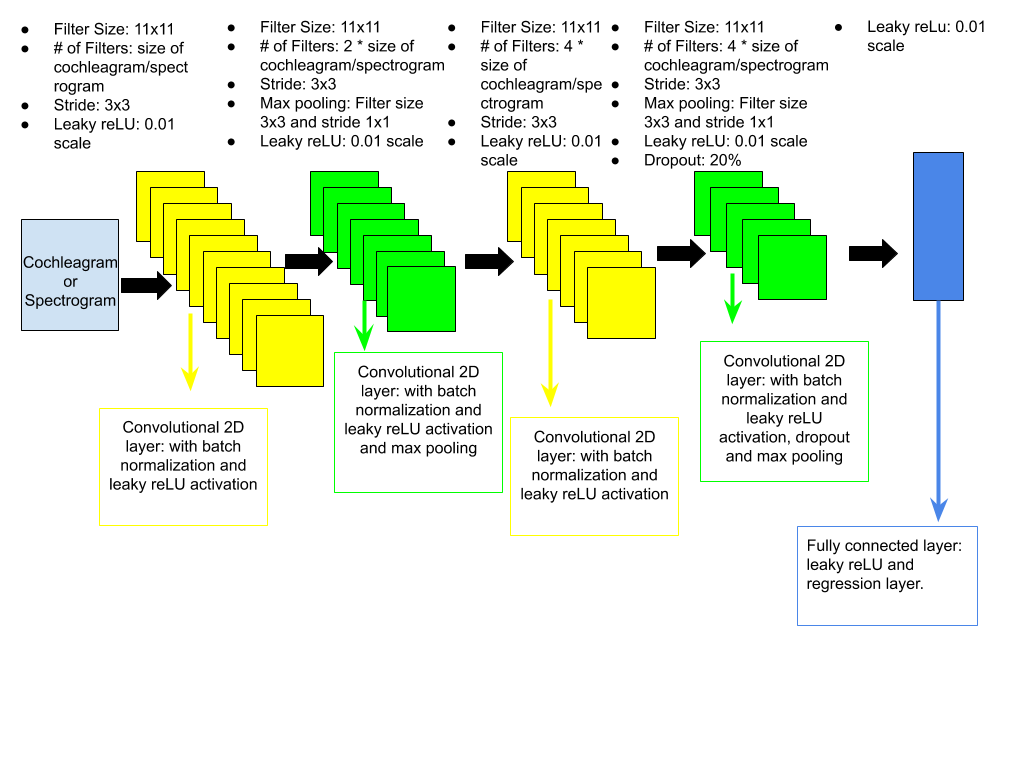
\includegraphics[width=1.2\linewidth]{cnn}
\caption{A CNN with 4 2-D Convolutional Layers and 2 downsampling 2-D Maxpooling Layers}
\label{fig:cnn}
\end{figure}
\begin{itemize}
\item \textbf{Image Input Layer}:\\
As described in the previous sections, this layer accepts the feature data as a 2-D or 3-D input. The number of neurons is this layer depends on the dimension size of the features. For cochleagram based training data, the number of input neurons are 64 and for spectrogram based training data, the number of input neurons are 121.

\item \textbf{Hidden Layers}:\\
Hidden layers in considered deep CNN were combination of \textbf{four} convolution2dLayer(s) with a downsampling by maxPooling2dLayer(s) after second and fourth convolution2dLayer respectively. The hidden layers had the following properties:
\begin{itemize}
\item \textbf{Convolution2dLayer}:\\
This is a 2-D convolutional layer which applies sliding convolutional filters to the input. The layer convolves the input by moving the filters along the input vertically and horizontally and computing the dot product of the weights and the input, and then adding a bias term. The convolutional \textbf{filter's kernel size} was kept at \textbf{11x11} and the \textbf{number of convolutional filters} were kept the \textbf{same as feature size i.e 64/121} for the \textbf{first} convolution2dLayer, \textbf{2x(feature size i.e 64/121)} for the \textbf{second} convolution2dLayer and \textbf{4x(feature size i.e 64/121)} for the \textbf{remaining two} convolution2dLayer(s).
\item \textbf{Batch Normalization}:
As discussed in the previous sections, this layer helps in overcoming “internal covariate shift” problem. It does so by normalizing the inputs of each layer.
\item \textbf{Leaky reLU activation}:\\
Using reLU activation often encounters a \enquote{\textit{Dying ReLU problem}} i.e. when inputs approach zero, or are negative, the gradient of the function becomes zero, the network cannot learn these inputs. Leaky reLU prevents the dying ReLU problem by making a slight variation on ReLU by having a small positive slope in the negative area (See figure: \ref{fig:leaky_relu}), so it does enable the network to learn, even for negative input values. The leaky reLU uses the following activation function to achieve this using the scale value of 0.01 as was considered in our implementation:
\[
  f(y) =
  \begin{cases}
    	y & \text{if $y>0$} \\
        0.01y & \text{otherwise} \\
  \end{cases}
\]
\begin{figure}[!htbp]
\centering
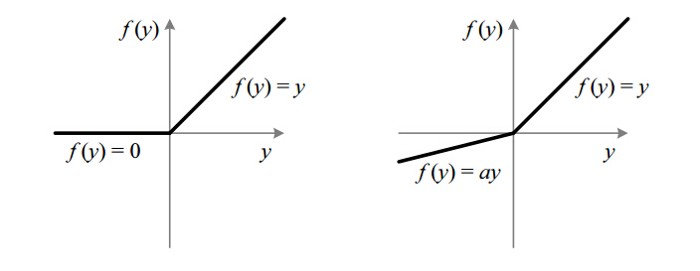
\includegraphics[width=1\linewidth]{leaky_relu}
\caption{Leaky reLU as compared to reLU}
\label{fig:leaky_relu}
\end{figure}
\item \textbf{MaxPooling2dLayer}:\\
This layer performs the down-sampling by dividing the input into rectangular pooling regions, and computing the maximum of each region. In our implementation, the max pooling filter of size \textbf{3x3} was considered.
\end{itemize}
\item \textbf{Output Layer}:\\
Output layer is a fully connected layer with leaky reLU activation and regression operation. For a spectrogram based IRM, the number of output neurons are 121 and for a cochleagram based IRM, the number of output neurons are 64. Regression operation tries to minimize a cost function to model the spectrogram/cochleagram with respect to the IRM to estimate. The metric used for optimisation is RMSE to minimize the intended cost function for modeling the training data.
\end{itemize}
\subsection{Experiments with the deep CNN}
The CNN was trained using spectrogram and cochleagram as training data. The intended training target for spectrogram was IRM based on spectrogram and for cochleagram was IRM based on cochleagram respectively. The performance analysis are as below:
\begin{itemize}
\item \textbf{Intelligibility}:\\
The STOI values for 0 and -2 SNR are documented in the table \ref{tab:cnn_stoi}. As per the information from this table following observations can be made:
\begin{enumerate}
\item \textbf{Comparison with the baseline DNN}:\\
For the best performing feature set, the gain in intelligibilty has been observed for CNN based learning model to be of \textbf{4.8\%} and \textbf{3.9\%} for 0 and -2 SNR respectively.
\item \textbf{Comparison between worst and best performing training data}:\\
The gain in intelligibility from the worst to the best performing training data is \textbf{8.8\%} and \textbf{5.3\%} for 0 and -2 SNR respectively. Since, only spectrogram and cochleagram was used as the training data, this is a comparison of intelligibility gain from spectrogram to cochleagram as training data.
\item \textbf{Intelligibility gain from the noisy mixture audios}:\\
The gain in intelligibility when considering the original noisy mixture (See table: \ref{tab:stoi_mix}) for the best performing training data was found out to be \textbf{17.8\%} and \textbf{19.4\%} for 0 and -2 SNR respectively.
\end{enumerate}
This points out that for cochleagram based training data and IRM based on the cochleagram the intelligibility gain is the best when compared to the previous learning models.
\begin{table}[!htbp]
\centering
\begin{tabular}{ |p{12cm}|p{1.7cm}|p{1.7cm}|  }
\hline
\textbf{Features} & \multicolumn{2}{|c|}{\textbf{STOI}} \\
\hline
\cellcolor{black} & SNR 0 & SNR -2\\
\hline
\rowcolor[HTML]{ADD8E6}Cochleagram	& 0.86	& 0.80\\
\hline
Spectrogram	& 0.79	& 0.76\\
\hline
\end{tabular}
\caption{STOI performance: CNN}
\label{tab:cnn_stoi}
\end{table}
\item \textbf{Quality}:\\
The PESQ values for 0 and -2 SNR are documented in the table \ref{tab:cnn_pesq}. As per the information from this table following observations can be made:
\begin{enumerate}
\item \textbf{Comparison with the baseline DNN}:\\
On comparing the tabulated data from the table \ref{tab:cnn_pesq}, with the baseline DNN's performance in the table \ref{tab:dnn_0_pesq_2}, for the best performing feature set, there is gain in quality by \enquote{\textbf{2.1\%}} for \textbf{PESQMOS} and \enquote{\textbf{6.7\%}} for \textbf{MOSLQO} at SNR 0. For SNR -2, the gain in quality is by \enquote{\textbf{2.2\%}} for \textbf{PESQMOS} and \enquote{\textbf{8\%}} for \textbf{MOSLQO}.
\item \textbf{Comparison between worst and best performing training data}:\\
The gain in quality from the worst to the best performing training data is
\enquote{\textbf{9\%}} for \textbf{PESQMOS} and \enquote{\textbf{14.5\%}} for \textbf{MOSLQO} at SNR 0. For SNR -2, the gain in quality is by \enquote{\textbf{12.3\%}} for \textbf{PESQMOS} and \enquote{\textbf{16.7\%}} for \textbf{MOSLQO}.
\item \textbf{Quality gain from the noisy mixture audios}:
On comapring with the quality of noisy mixtures as tabulated in the table \ref{tab:pesq_mix}, the gain in quality is found out to be \enquote{\textbf{15.2\%}} for \textbf{PESQMOS} and \enquote{\textbf{20.7\%}} for \textbf{MOSLQO} for SNR 0. For SNR -2, the gain in quality is by \enquote{\textbf{15.6\%}} for \textbf{PESQMOS} and \enquote{\textbf{22.4\%}} for \textbf{MOSLQO} respectively.\\
This again points out that for cochleagram based training data and IRM based on the cochleagram the quality gain is the best when compared to the previous learning models. 
\end{enumerate}
\begin{table}[!htbp]
\centering
\begin{tabular}{ |p{8cm}|p{1.7cm}|p{1.7cm}|p{1.7cm}|p{1.7cm}|  }
\hline
\textbf{Features} & \multicolumn{4}{|c|}{\textbf{PESQ}}\\
\hline
\cellcolor{black} & \multicolumn{2}{|c|}{SNR 0} & \multicolumn{2}{|c|}{SNR -2}\\
\hline
\cellcolor{black} & PESQMOS & MOSLQO & PESQMOS & MOSLQO\\
\hline
\cellcolor[HTML]{ADD8E6}Cochleagram	& \cellcolor[HTML]{ADD8E6}2.50	& \cellcolor[HTML]{ADD8E6}2.21	& \cellcolor{yellow}2.38	& \cellcolor{yellow}2.16\\
\hline
Spectrogram	& 2.22	& 1.93	& 2.10	& 1.85\\
\hline
\end{tabular}
\caption{PESQ performance: CNN}
\label{tab:cnn_pesq}
\end{table}
\end{itemize}
% Chapter 4
\chapter{Performance Analysis and Conclusions} % Main chapter title

\label{Chapter4} % For referencing the chapter elsewhere, use \ref{Chapter4} 

%----------------------------------------------------------------------------------------

\section{Intelligibility Analysis}
On comparing the best performing training data for the three deep learning models as discussed in the chapter \ref{Chapter3}, the gain in the intelligibility can be tabulated as below:\\
\begin{table}[!htbp]
\centering
\begin{tabular}{|p{8cm}|p{4cm}|p{4cm}|}
\hline
\textbf{Deep Learning Model} & \textbf{STOI Gain at 0 SNR} & \textbf{STOI Gain at -2 SNR}\\
\hline
Baseline DNN & 12.3\% & 14.9\%\\
\hline
DNN with biased sigmoid activation & 9.6\% & 14.9\%\\
\hline
CNN with leaky reLU & 17.8\% & 19.4\%\\
\hline
\end{tabular}
\caption{Intelligibility Gains}
\label{tab:i_gain_compare}
\end{table}
\\
Hence, from \ref{tab:i_gain_compare} and observing the intelligibility scores of original noisy mixtures from the table \ref{tab:stoi_mix}, we can make following analysis:\\
\begin{itemize}
\item STOI for original noisy mixture at 0 SNR is 0.73. This is already a decent score (on the STOI metric scale of 0-1) and hence, the subsequent gain in intelligibility at 0 SNR post speech enhancement is lower than the STOI gain at -2 SNR for which the original noisy mixture has a STOI score of 0.67.
\item There is a clear trend of improvement of STOI gain from the noisy audio mixtures at 0 SNR to the noisy audio mixtures at -2 SNR. This affirms the ability of IRM in preserving the clean speech energies which is helpful for speech enhancement particularly in low SNR scenarios.
\item Second DNN with the biased sigmoid activation provides less gain in intelligibility scores for 0 SNR and the same score of intelligibility for the -2 SNR when compared to the baseline DNN. It's intelligibility gain when compare to the CNN based model is however poor. Using baseline DNN as a reference, for the dataset considered, the prima facie trend show slightly poor performance of the biased sigmoid layer comapred to the reLU activation used in the baseline. But, to make a conclusive remark training on a larger dataset would be required. 
\item CNN with leaky reLU shows the best intelligibility gains among the three considered deep learning models and also places the least demand on the feature extraction as only spectrogram/cochleagram were used in the training phase.
\item For DNN based learning models and the spectrogram based training target, the better performing feature set was always found to include the gammatone cepstral features i.e. the set \enquote{\textit{GFCC, GFCC delta, GFCC delta delta}}. However, for the training target based on cochleagram, the best performing feature set was always found to include the feature set  \enquote{\textit{Cochleagram}}.
\end{itemize}
%---------------------------------------------------------------------------
\section{Quality Analysis}
On comparing the best performing training data for the three deep learning models as discussed in the previous chapter \ref{Chapter3}, the gain in the quality scores considering MOSLQO has been tabulated in the table \ref{tab:q_gain_compare}. MOSLQO is chosen over PESQMOS as it defines perceptual quality gain with respect to the human listening objectivity.\\
\begin{table}[!htbp]
\centering
\begin{tabular}{|p{8cm}|p{3cm}|p{4cm}|}
\hline
\textbf{Deep Learning Model} & \textbf{Quality Gain at 0 SNR} & \textbf{Quality Gain at -2 SNR}\\
\hline
Baseline DNN & 13.1\% & 15.6\%\\
\hline
DNN with biased sigmoid activation  & 12.9\% & 13.8\%\\
\hline
CNN with leaky reLU & 20.7\% & 22.4\%\\
\hline
\end{tabular}
\caption{Quality Gains}
\label{tab:q_gain_compare}
\end{table}

Hence from the tables \ref{tab:q_gain_compare} and \ref{tab:pesq_mix}, the following analysis can be made for quality as a performance metric:
\begin{itemize}
\item MOSLQO scores for original noisy mixture at 0 SNR is 1.83. This is qualitatively at the lower scale of 1-5 for MOSLQO. The subsequent gain in quality metric at 0 SNR shows an improvement of 15.6\% on average. Likewise, quality scores at -2 SNR for original noisy mixtures is 1.73, but the quality gain is higher as compared to the 0 SNR case with an average gain of 17.2\%. This points out, and as also observed from all three learning models, the speech enhancement has more scope of audio quality improvement at the lower SNR levels when using IRM as the training target. 
\item DNN with biased sigmoid activation provides the least gain in the quality among the three deep learning models considered and hence, strengthen the argument that the reLU activation considered in the baseline DNN performs better than the biased sigmoid activation. However, to conclusively make this statement and as per the analysis from the intelligibility gains, training of both models on a larger dataset would be required.
\item CNN with leaky reLU shows the best quality gains among the three considered deep learning models along with the intelligibility as previously observed and also places the least demand on the feature extraction. This reaffirms the ability of this category of deep learning machines in better speech enhancement as compared to the other models.
\end{itemize}
%---------------------------------------------------------------------------
\section{\textbf{Conclusions}}
Based on study of the experiments conducted the following conclusions can be made:
\begin{itemize}
\item DNN based learning models perform better with cochleagram as training data and IRM based on cochleagram as the training target when compared with audio features and IRM based on spectrogram.
\item Using the feature set \enquote{GFCC, GFCC delta, GFCC delta delta} has the best performance for 0 SNR with DNN based learning models and IRM based on spectrogram as the training target.
\item Using the feature set \enquote{GFCC, GFCC delta, GFCC delta delta, Spectrogram} has the best performance for -2 SNR with DNN based learning models and IRM based on spectrogram as the training target. 
\item This highlights the importance of gammatone based cepstral features in speech enhancement where the learning machine places a significant demand on feature extraction as a part of training data.
\item CNN with leaky reLU activation has the best performance in terms of gains in intelligibility and quality scores out of all considered models. \item Performance of CNN also underlines the importance and power of this category of learning machines which have the ability to learn the patterns in the training data by themselves thus placing minimum demand on feature extraction. 
\item It's also noteworthy that the improvement in gain of both intelligibility and quality post speech enhancement is more in -2 SNR as compared to 0 SNR. Hence, for noisy mixtures with even lower SNR values, the scope of intelligibility and quality gain is established as per the observed trends from the experiments.
\end{itemize}
%---------------------------------------------------------------------------
\section{\textbf{Future Prospects}}
\begin{itemize}
\item \textbf{Train on larger dataset}:\\
All of the considered models were trained on the TIMIT dataset of 1718 audio samples. Hence, by expanding the dataset all of the models can be trained to generalize and learn \enquote{noise} from the noisy mixtures more efficiently thus helping in better speech enhancement and source separation. This can thus help in improvement of intelligibility and quality gains.\\ This would also help in conclusively answering the argument regarding the performance of the biased sigmoid layer with respect to the reLU layer.
\item \textbf{Train on lower SNR values}:\\
All of the considered models were trained for noisy mixtures at 0 and -2 SNR respectively. As per the analysis of performanc metrics, the gain in quality and intelligibility was more for noisy mixtures at -2 SNR post enhancement. By testing on noisy mixtures at even lower SNRs, this trend can be verified.
\item \textbf{Scale to binaural models}:\\ Using the Interaural Time Difference (ITD) and Interaural Intensity Difference(IID) as additional features, these models can be trained for binaural mixtures.
\item \textbf{Testing on more models}:\\ This involves exploring unsupervised learning as standalone or in tandem with the supervised learning  to check for any improvement in performance metrics.
\item \textbf{Weight Initialization}:\\ In the models implemented, the weights are uninitialized before training. This allowed the deep learning models to self initialize the weights randomly. Using unsupervised pretraining first, weights can be appropriately initialised to ensure fast arrival to the optimisation point during training.
\item \textbf{Real-time application}:\\ For the models and feature sets considered, there is an average latency of around 0.25 s during prediction phase from the time of feature extraction to the enhanced speech's reconstruction. This is when the testing dataset is readily available. For a real-time application which would involve binarization of the audio recording for storage first to the signal reconstruction post speech enhancement, there is enough potential for optimising the models for reducing latency further.
\item \textbf{Transfer Learning}:\\ Comparison of the performance evaluation for the models considered in the project with the well known neural networks like GoogLeNet , Alexnet etc can also be studied.
\end{itemize} 

%----------------------------------------------------------------------------------------
%	REPORT CONTENT - APPENDICES
%----------------------------------------------------------------------------------------

\appendix % Cue to tell LaTeX that the following "chapters" are Appendices

% Include the appendices of the thesis as separate files from the Appendices folder

% Appendix A

\chapter{Performance Metrics} % Main appendix title

\label{AppendixA} % For referencing this appendix elsewhere, use \ref{AppendixA}

\section{STOI}
\textit{\textbf{Short-Time Objective Intelligibility (STOI)}, measures the correlation between the short-time temporal envelopes of a reference (clean) audio signal and a degraded audio signal for speech intelligibility of human speech \cite{ref:ieee_stoi}. The value range of STOI is typically between 0 and 1, 0 being the worst and 1 being the best intelligibility. STOI values can also be considered to be percentage correct.}

\section{PESQ}
\textit{\textbf{Perceptual Evaluation of Speech Quality (PESQ)} is the standard metric recommended by the International Telecommunication Union (ITU) for analysing quality of a degraded signal with respect to a clean reference signal \cite{ref:pesq}. PESQ applies an auditory transform to produce a loudness spectrum, and compares the loudness spectra of a clean reference signal and a degraded signal to produce a score in a range of negative 0.5 to 4.5. This score is regarded to be a Mean Opinion Score (MOS). MOS can further be transformed in terms of listening objectivity metrics on a scale from 0 to 5 known as Listening Quality Objectivity (LQO). LQO scale is important as it is a mapping from MOS as per the human auditory response.}


%----------------------------------------------------------------------------------------
%	BIBLIOGRAPHY
%----------------------------------------------------------------------------------------

\printbibliography[title = Bibliography]

%----------------------------------------------------------------------------------------

\end{document}  
